\chapter{Results and Discussion}\label{ch:results_and_discussion}
% ---What Changes Where, and Does It Matter?

In line with the thesis objective---\emph{to characterize how visual instruction tuning reshapes the LLaVA backbone and how the representational changes affect multimodal performance}---this chapter presents the experimental results. Each section corresponds to one methodological block from Chapter~\ref{ch:methodology} and links the findings directly to the research questions introduced in Chapter~\ref{ch:introduction}.

The chapter begins with a broad view of models' performance and representation similarity at different levels of the residual stream. It then moves to a finer-grained analysis of the geometry of data representations. Finally, a functional inspection of the LLaVA backbone through layer patching validates and contextualizes the earlier results.

\section{Zero-shot QA: Performance Effects of Visual Instruction Tuning}

Before examining internal changes in the LLaVA backbone, we first quantify the performance impact of visual instruction tuning across text and multimodal QA tasks. We compare zero-shot accuracy of the fine-tuned checkpoint to the pretrained one---which is LLaVA with just feature alignment and Vicuna v1.5 7B as the LLM backbone (see Sections~\ref{sec:llava} and \ref{sec:residual_stream_extraction_method})---on the benchmarks described in Section~\ref{sec:question_answering}.

Table~\ref{tab:benchmark_comparison} summarizes the results. The fine-tuned model outperforms the pretrained model on every dataset. The largest gain is on COCOVQA, especially on the multimodal subset, where accuracy rises by $\sim$ 58\% relative to the pretrained model (41.88\%). On COCOVQA, both checkpoints score higher on text than on multimodal (58.36\% vs. 41.88\%); the fine-tuned model roughly halves this difference (from 16.75\% to 8.04\%). Coincidentally, on ScienceQA, the fine-tuned model achieves the same accuracy on the text and multimodal subsets (both 66.53\%).

\begin{table}
\centering
\begin{tabular}{lccc}
\toprule
\textbf{Benchmark} & \textbf{Modality} & \textbf{Pretrained LLaVA} & \textbf{LLaVA} \\
\midrule
MMLU & Text & 48.67\% & \textbf{50.63\%} \\
ScienceQA & Text & 64.25\% & \textbf{66.53\%} \\
ScienceQA & Multimodal & 58.11\% & \textbf{66.53\%} \\
COCOVQA & Text & 58.36\% & \textbf{74.56\%} \\
COCOVQA & Multimodal & 41.88\% & \textbf{66.52\%} \\
\bottomrule
\end{tabular}
\caption{
    Zero-shot accuracy (\%) of the pretrained and fine-tuned LLaVA (v1.5 7B) on MMLU, ScienceQA (text and multimodal), and COCOVQA (text and multimodal).
}
\label{tab:benchmark_comparison}
\end{table} 

\paragraph{Prompting and format sensitivity.}

Careful prompt formatting---e.g., instructing the model to ``\emph{answer with a single word or phrase}''---improves zero-shot performance for both checkpoints, as noted in the LLaVA reports \cite{liuImprovedBaselinesVisual2024} and prompt-engineering studies \cite{weiChainofThoughtPromptingElicits2023, chenUnleashingPotentialPrompt2024}. On MMLU, aligning the prompt with training-time formats helps reconcile differences with prior reports for Vicuna (LLaVA pretrained LLM backbone) and LLaMA-2 (Vicuna pretrained LLM backbone) \cite{touvronLlama2Open2023,zhengJudgingLLMasaJudgeMTBench, doimoRepresentationLandscapeFewShot}, which can vary with few-shot setup and inference instructions. We explored alternative prompt formats and the fine-tuned model is more robust and maintains higher zero-shot accuracy across these variants. Beyond multimodal inputs, visual instruction tuning also benefits purely textual QA, consistent with LLaVA's rich instruction data (descriptions, dialogue structure, reasoning steps; see Section~\ref{sec:llava}). Our ScienceQA multimodal accuracy (66.53\%) closely matches LLaVA-1.5 7B reports (66.8\%) \cite{llava_model_zoo}. On COCOVQA, the fine-tuned model exceeds classic pre-Transformer VQA systems \cite{renExploringModelsData2015, luHierarchicalQuestionImageCoAttention2017}, whereas the pretrained checkpoint does not.

\paragraph{Task type matters (open-ended vs.\ multiple-choice).}

Gains are modest on MMLU and ScienceQA but substantial on COCOVQA. A likely reason is the \emph{match} between training objectives and evaluation format: LLaMA-2/Vicuna training and evaluation emphasize multiple-choice datasets \cite{touvronLlama2Open2023,zhengJudgingLLMasaJudgeMTBench} (PIQA, SIQA, HellaSwag, WinoGrande, OBQA, CSQA, MMLU), whereas LLaVA's instruction tuning includes open-ended VQA and caption-style supervision \cite{liuVisualInstructionTuning2023,liuImprovedBaselinesVisual2024} (VQAv2, GQA, OKVQA, OCR-VQA). Since the LLaVA backbone inherits from LLaMA-2 and Vicuna, which were trained on multiple-choice datasets, improvements on such datasets remain modest. By contrast, LLaVA's fine-tuning on open-ended tasks yields much larger gains. Consistent with this, the pretrained model (a LLaMA-2 descendant) typically scores lower on open-ended QA than on multiple-choice, and the largest fine-tuning deltas appear on the open-ended COCOVQA subsets.

\medskip
These behavioral patterns motivate the representational analyses that follow: \emph{where in the backbone do these fine-tuning gains arise, how are text and image information integrated with depth, and how are they reflected in the internal geometry of the model?}

\section{Where the Backbone Changes: Representational Similarity}\label{sec:representational_similarity}

We compare residual-stream representations of the fine-tuned and pretrained LLaVA at two levels of granularity: (i) \emph{layer outputs} and (ii) \emph{per-head attention projections} (Section~\ref{sec:residual_stream_extraction_method}). Similarities are measured using Neighborhood Overlap (NO) and Linear CKA (see Section~\ref{sec:similarity_measures}) on embeddings extracted from the COCOVQA dataset in text and visual QA settings (Section~\ref{sec:question_answering}). This analysis reveals \emph{where} across depth and \emph{which} heads undergo the largest changes after fine-tuning.

\paragraph{Coarse-grained: similarity at the layers level.}

Figure~\ref{fig:layer_wise_similarity_cocovqa_combined} shows layer-wise residual stream similarity between the fine-tuned and pretrained checkpoints. Both NO and Linear CKA indicate substantial representational change (values well below 1). Across depth, text representations are consistently more similar than multimodal ones. In both metrics, similarity decreases sharply in the early layers, reaching a minimum around layer 7 for multimodal data, before gradually recovering toward the deeper layers. Similar trends were observed between the text and visual QA representations on ScienceQA.

\begin{figure}
    \centering
    \begin{subfigure}[t]{0.66\textwidth}
        \centering
        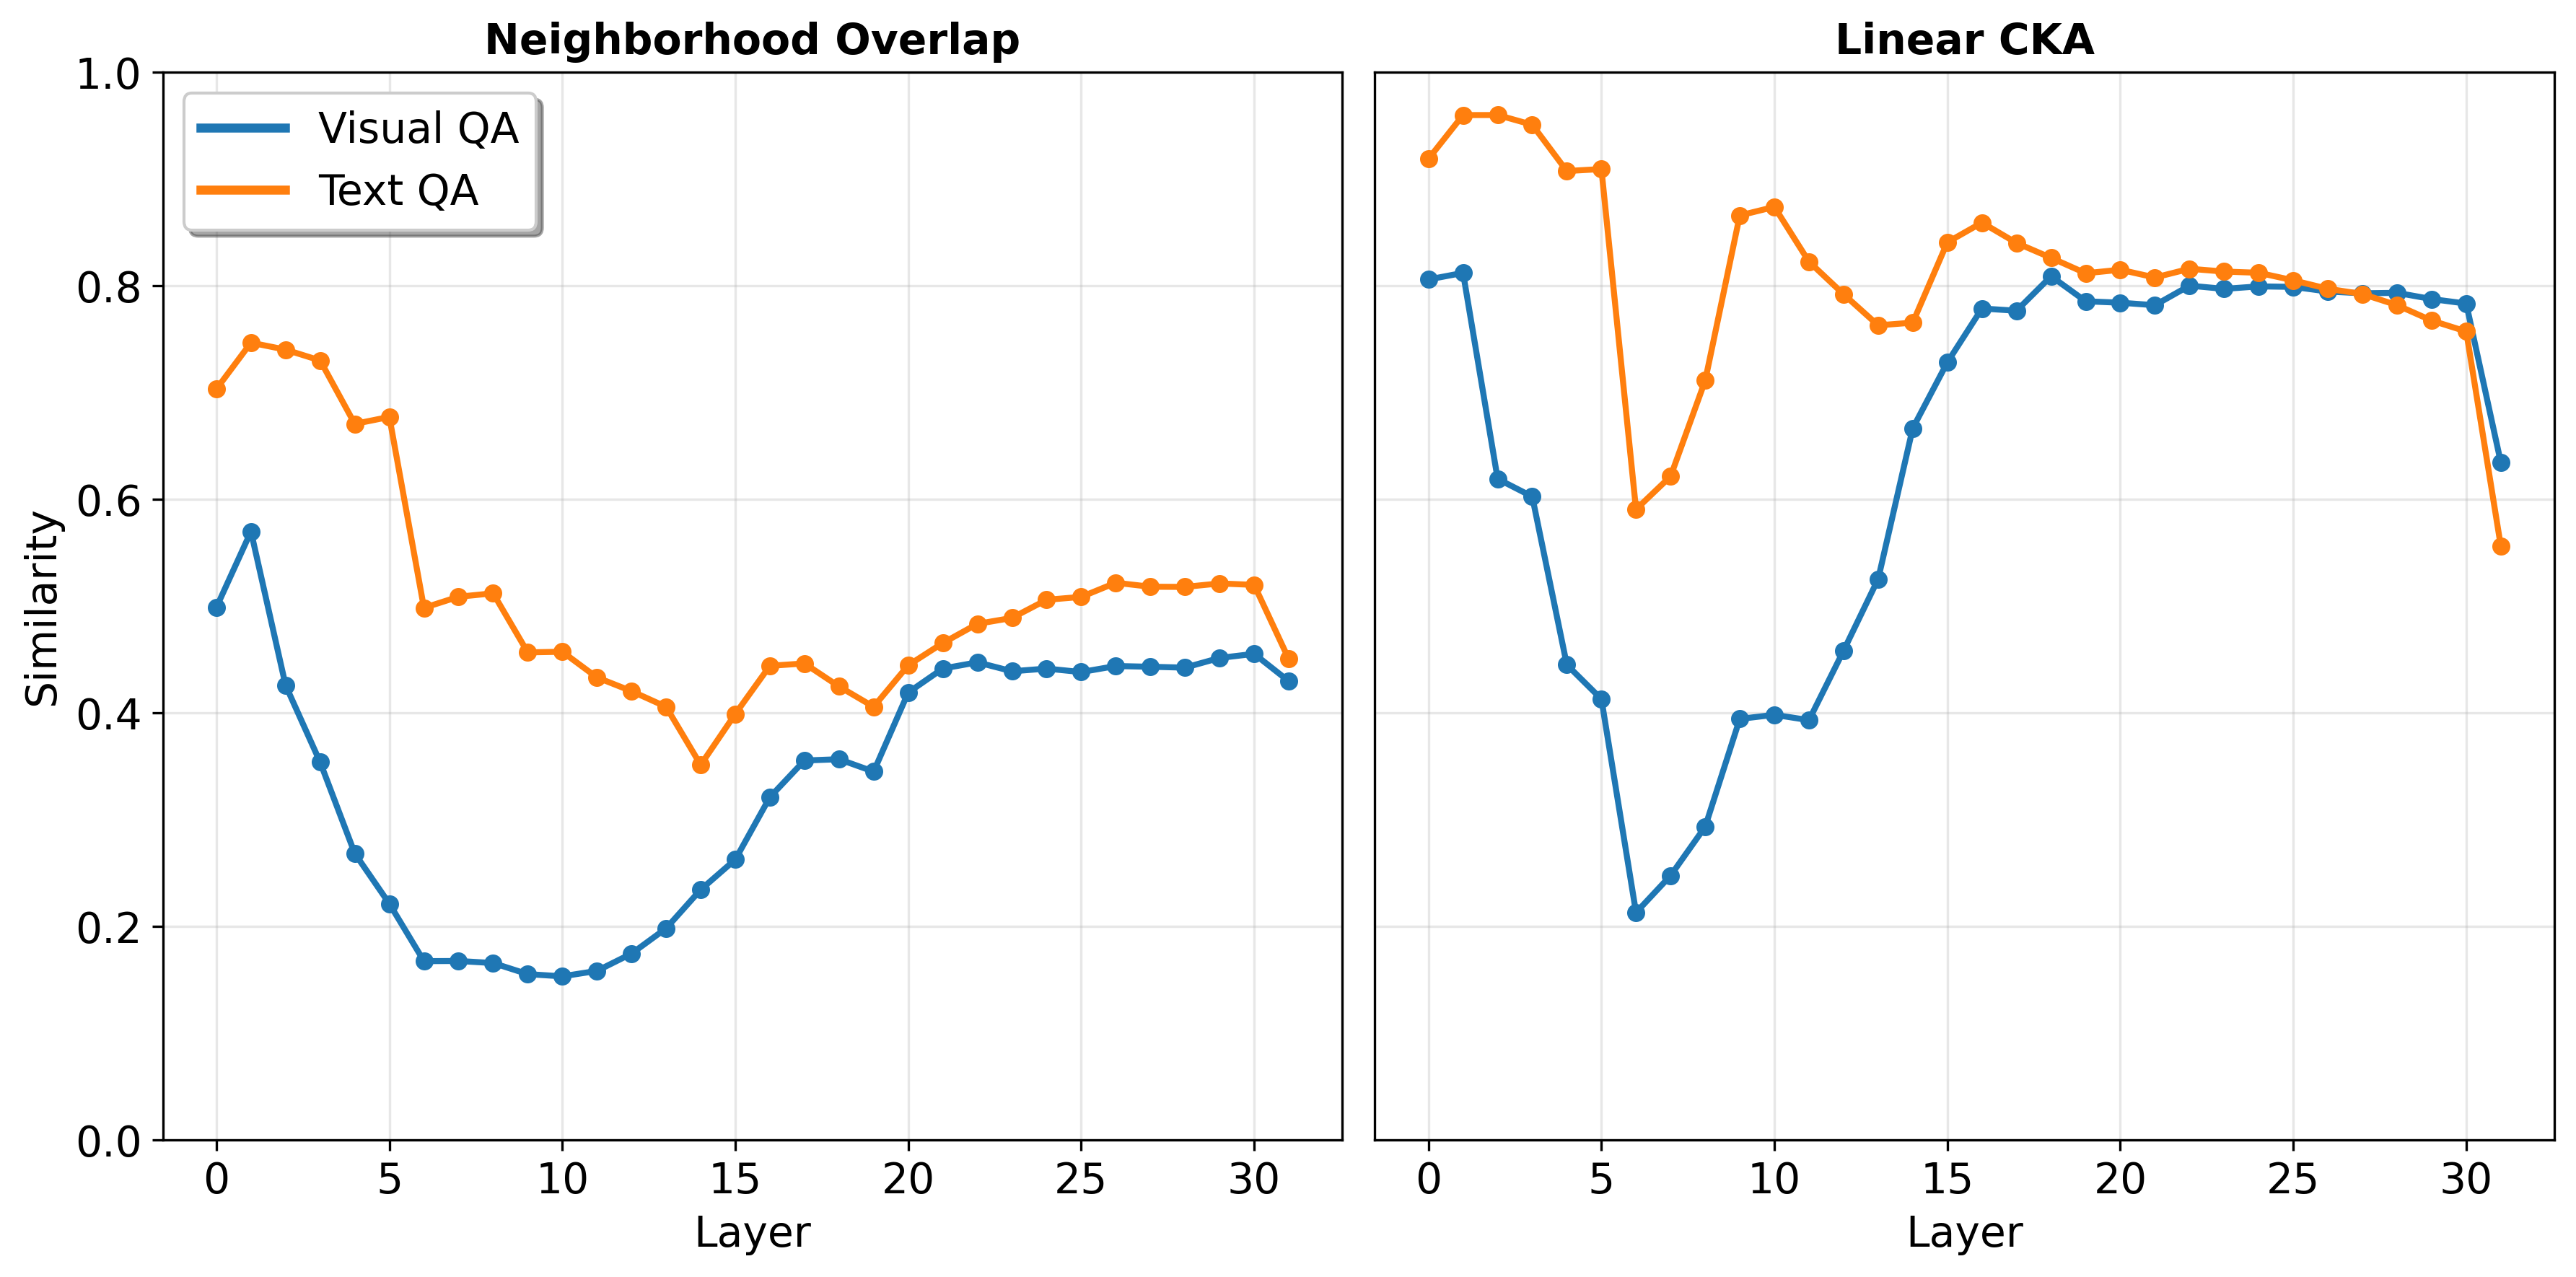
\includegraphics[width=\textwidth]{../images/chapter3/similarity_measures_output_layer_last_neighborhood_overlap_linear_cka.png}
        \vspace{-0.65cm}
        \caption{
            % leave caption blank
        }
        \label{fig:layer_wise_similarity_cocovqa_combined}
    \end{subfigure}
    \begin{subfigure}[t]{0.33\textwidth}
        \centering
        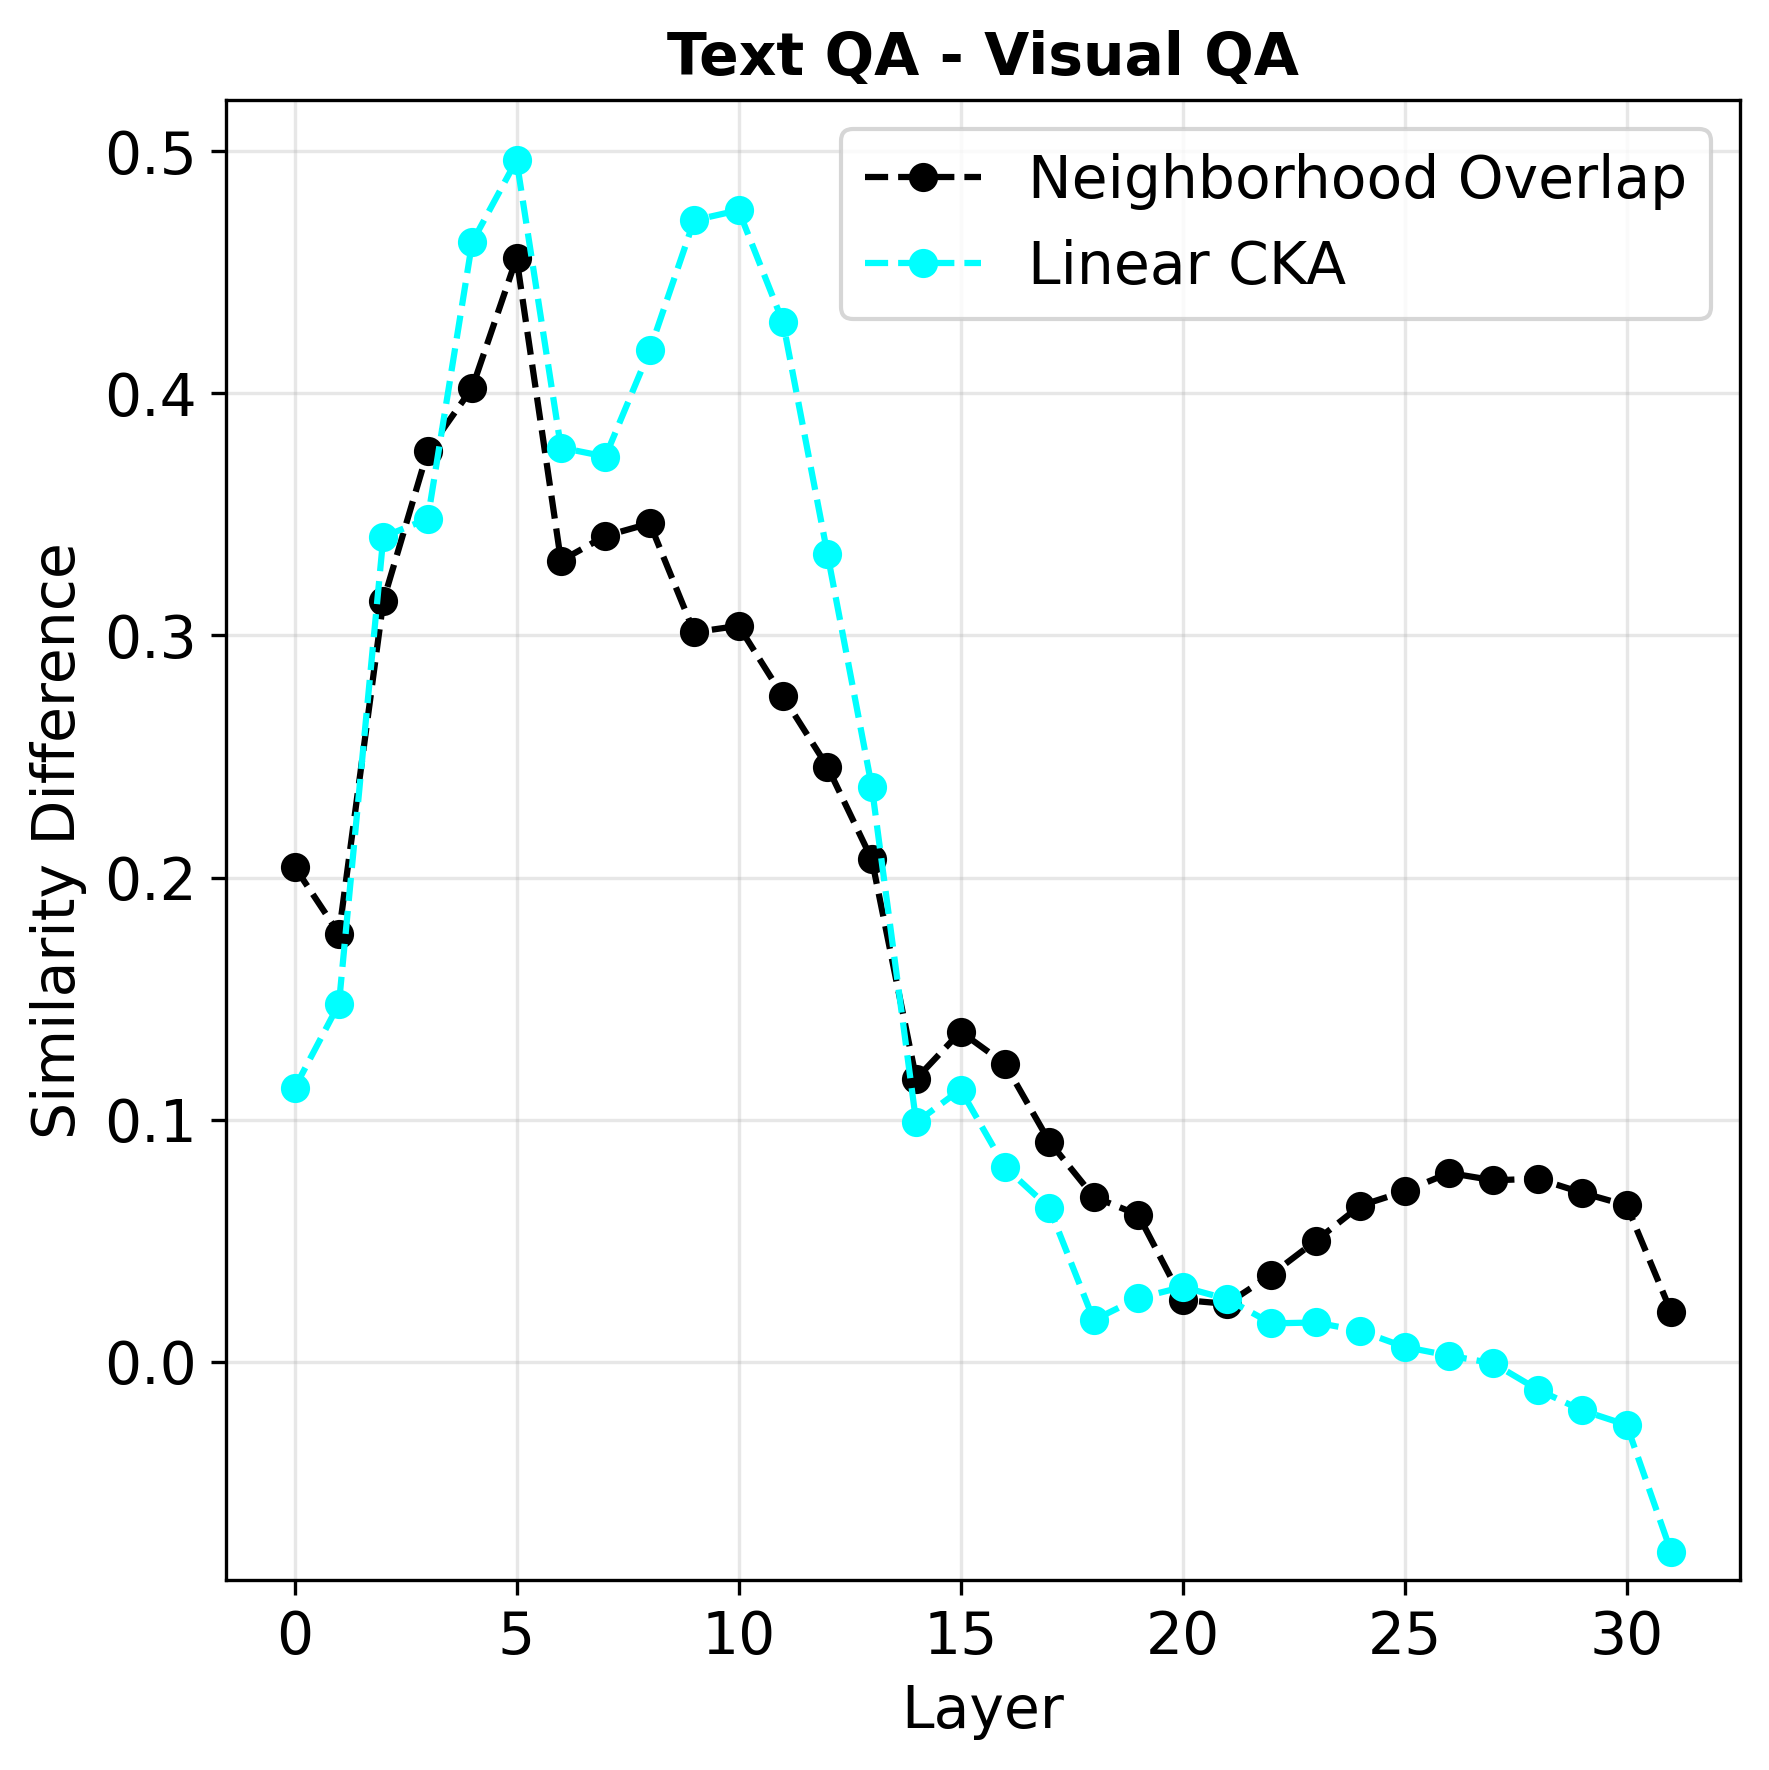
\includegraphics[width=\textwidth]{../images/chapter3/similarity_difference_measures_output_layer_last.png}
        \vspace{-0.65cm}
        \caption{
            % leave caption blank
        }
        \label{fig:layer_wise_similarity_cocovqa_difference}
    \end{subfigure}
    \vspace{-0.3cm}
    \caption{
        Layer-wise similarity between fine-tuned and pretrained LLaVA. 
        (a) NO (left) and Linear CKA (right) text (orange) and visual (blue) QA on COCOVQA. Higher values indicate greater cross-checkpoint similarity. 
        (b) Text-multimodal difference (black: NO, cyan: linear CKA); positive values mean higher similarity on text than on multimodal representations.
    }
    \label{fig:layer_wise_similarity_cocovqa}
\end{figure}


The difference curves in Figure~\ref{fig:layer_wise_similarity_cocovqa_difference}, showing the difference between text and multimodal similarity, \emph{though not standard}, highlights this contrast more directly and makes the underlying pattern easier to compare. The difference grows in early layers, peaking near layer 6 at $\sim$0.46-0.50 (NO/linear CKA), then steadily shrinks; by layer 21 the NO difference is near zero. In the final layers, Linear CKA becomes slightly negative, indicating that under this metric, multimodal representations across checkpoints are marginally more similar than their text representations.

\paragraph{Fine-grained: similarity at the heads level.}

While layer-wise similarity localizes the impact of fine-tuning by depth. To resolve where changes occur within a layer, we analyze the \emph{head-wise} residual stream similarity between the pretrained and fine-tuned models, quantifying how effects distribute across heads and whether they concentrate in specific heads.

Figure~\ref{fig:heads_wise_similarity_cocovqa_combined} reports head-wise NO at the attention output projected onto the residual stream (see Section~\ref{sec:residual_stream_extraction_method}). The layer-wise pattern repeats at head resolution: similarity on text exceeds multimodal, especially in early layers. Compared to text, fewer heads exhibit high similarity on multimodal data; this is clearest in the first two layers, where the text maximum (0.91) is surrounded by heads whose values are close to the multimodal maximum (0.79). Notably the maximum for both modalities occurs at layer 1, head 30. Additionally, some heads show comparable similarity across modalities (e.g., around head 27 in early layers). Linear CKA yielded consistent results.

The difference matrix in Figure~\ref{fig:heads_wise_similarity_cocovqa_difference} (head-wise analogue of Figure~\ref{fig:layer_wise_similarity_cocovqa_difference}) shows sparse heads where multimodal similarity exceeds text by up to $\sim$0.2 (negative values). In early layers (3-11), many heads are more similar on text than on multimodal data (up to $\sim$0.5). The mean across heads per layer, and its text-multimodal difference (Figure~\ref{fig:layer_wise_similarity_cocovqa_mean_heads}), aligns with the layer-wise curves. Similar results were observed between the text and visual QA representations on ScienceQA.

\begin{figure}
    \centering
    \begin{subfigure}[t]{\textwidth}
        \centering
        \vspace{-0.7cm}
        \caption{
            % leave caption blank
        }
        \label{fig:heads_wise_similarity_cocovqa_combined}
        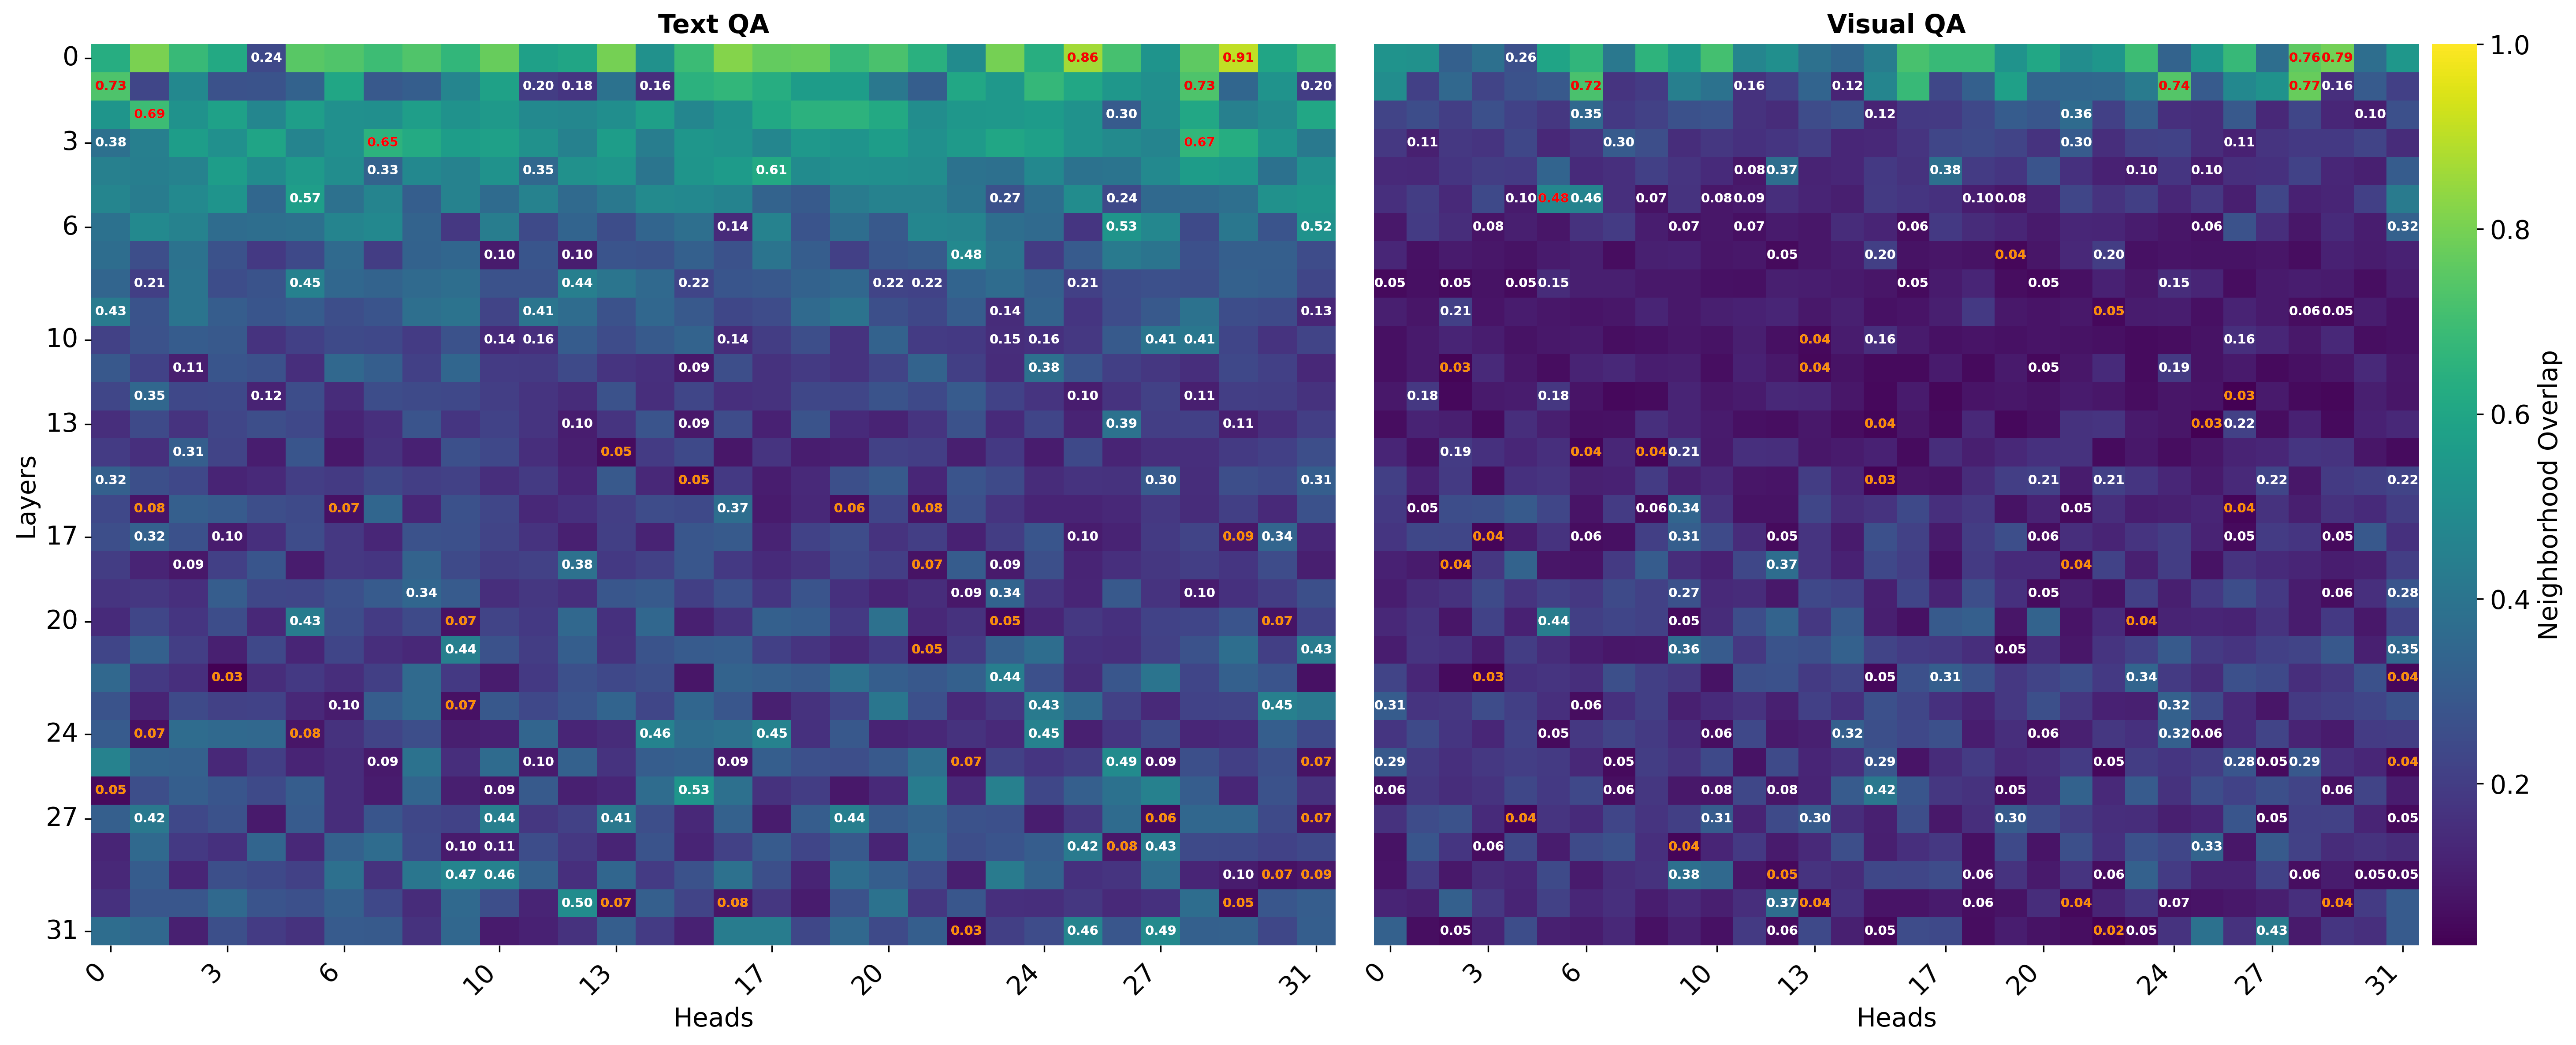
\includegraphics[width=\textwidth]{../images/chapter3/similarity_matrix_combined_neighborhood_overlap.png}
    \end{subfigure}
    
    \vspace{0.5cm}
    
    \begin{subfigure}[t]{0.6\textwidth}
        \centering
        \vspace{-0.7cm}
        \caption{
            % leave caption blank
        }
        \label{fig:heads_wise_similarity_cocovqa_difference}
        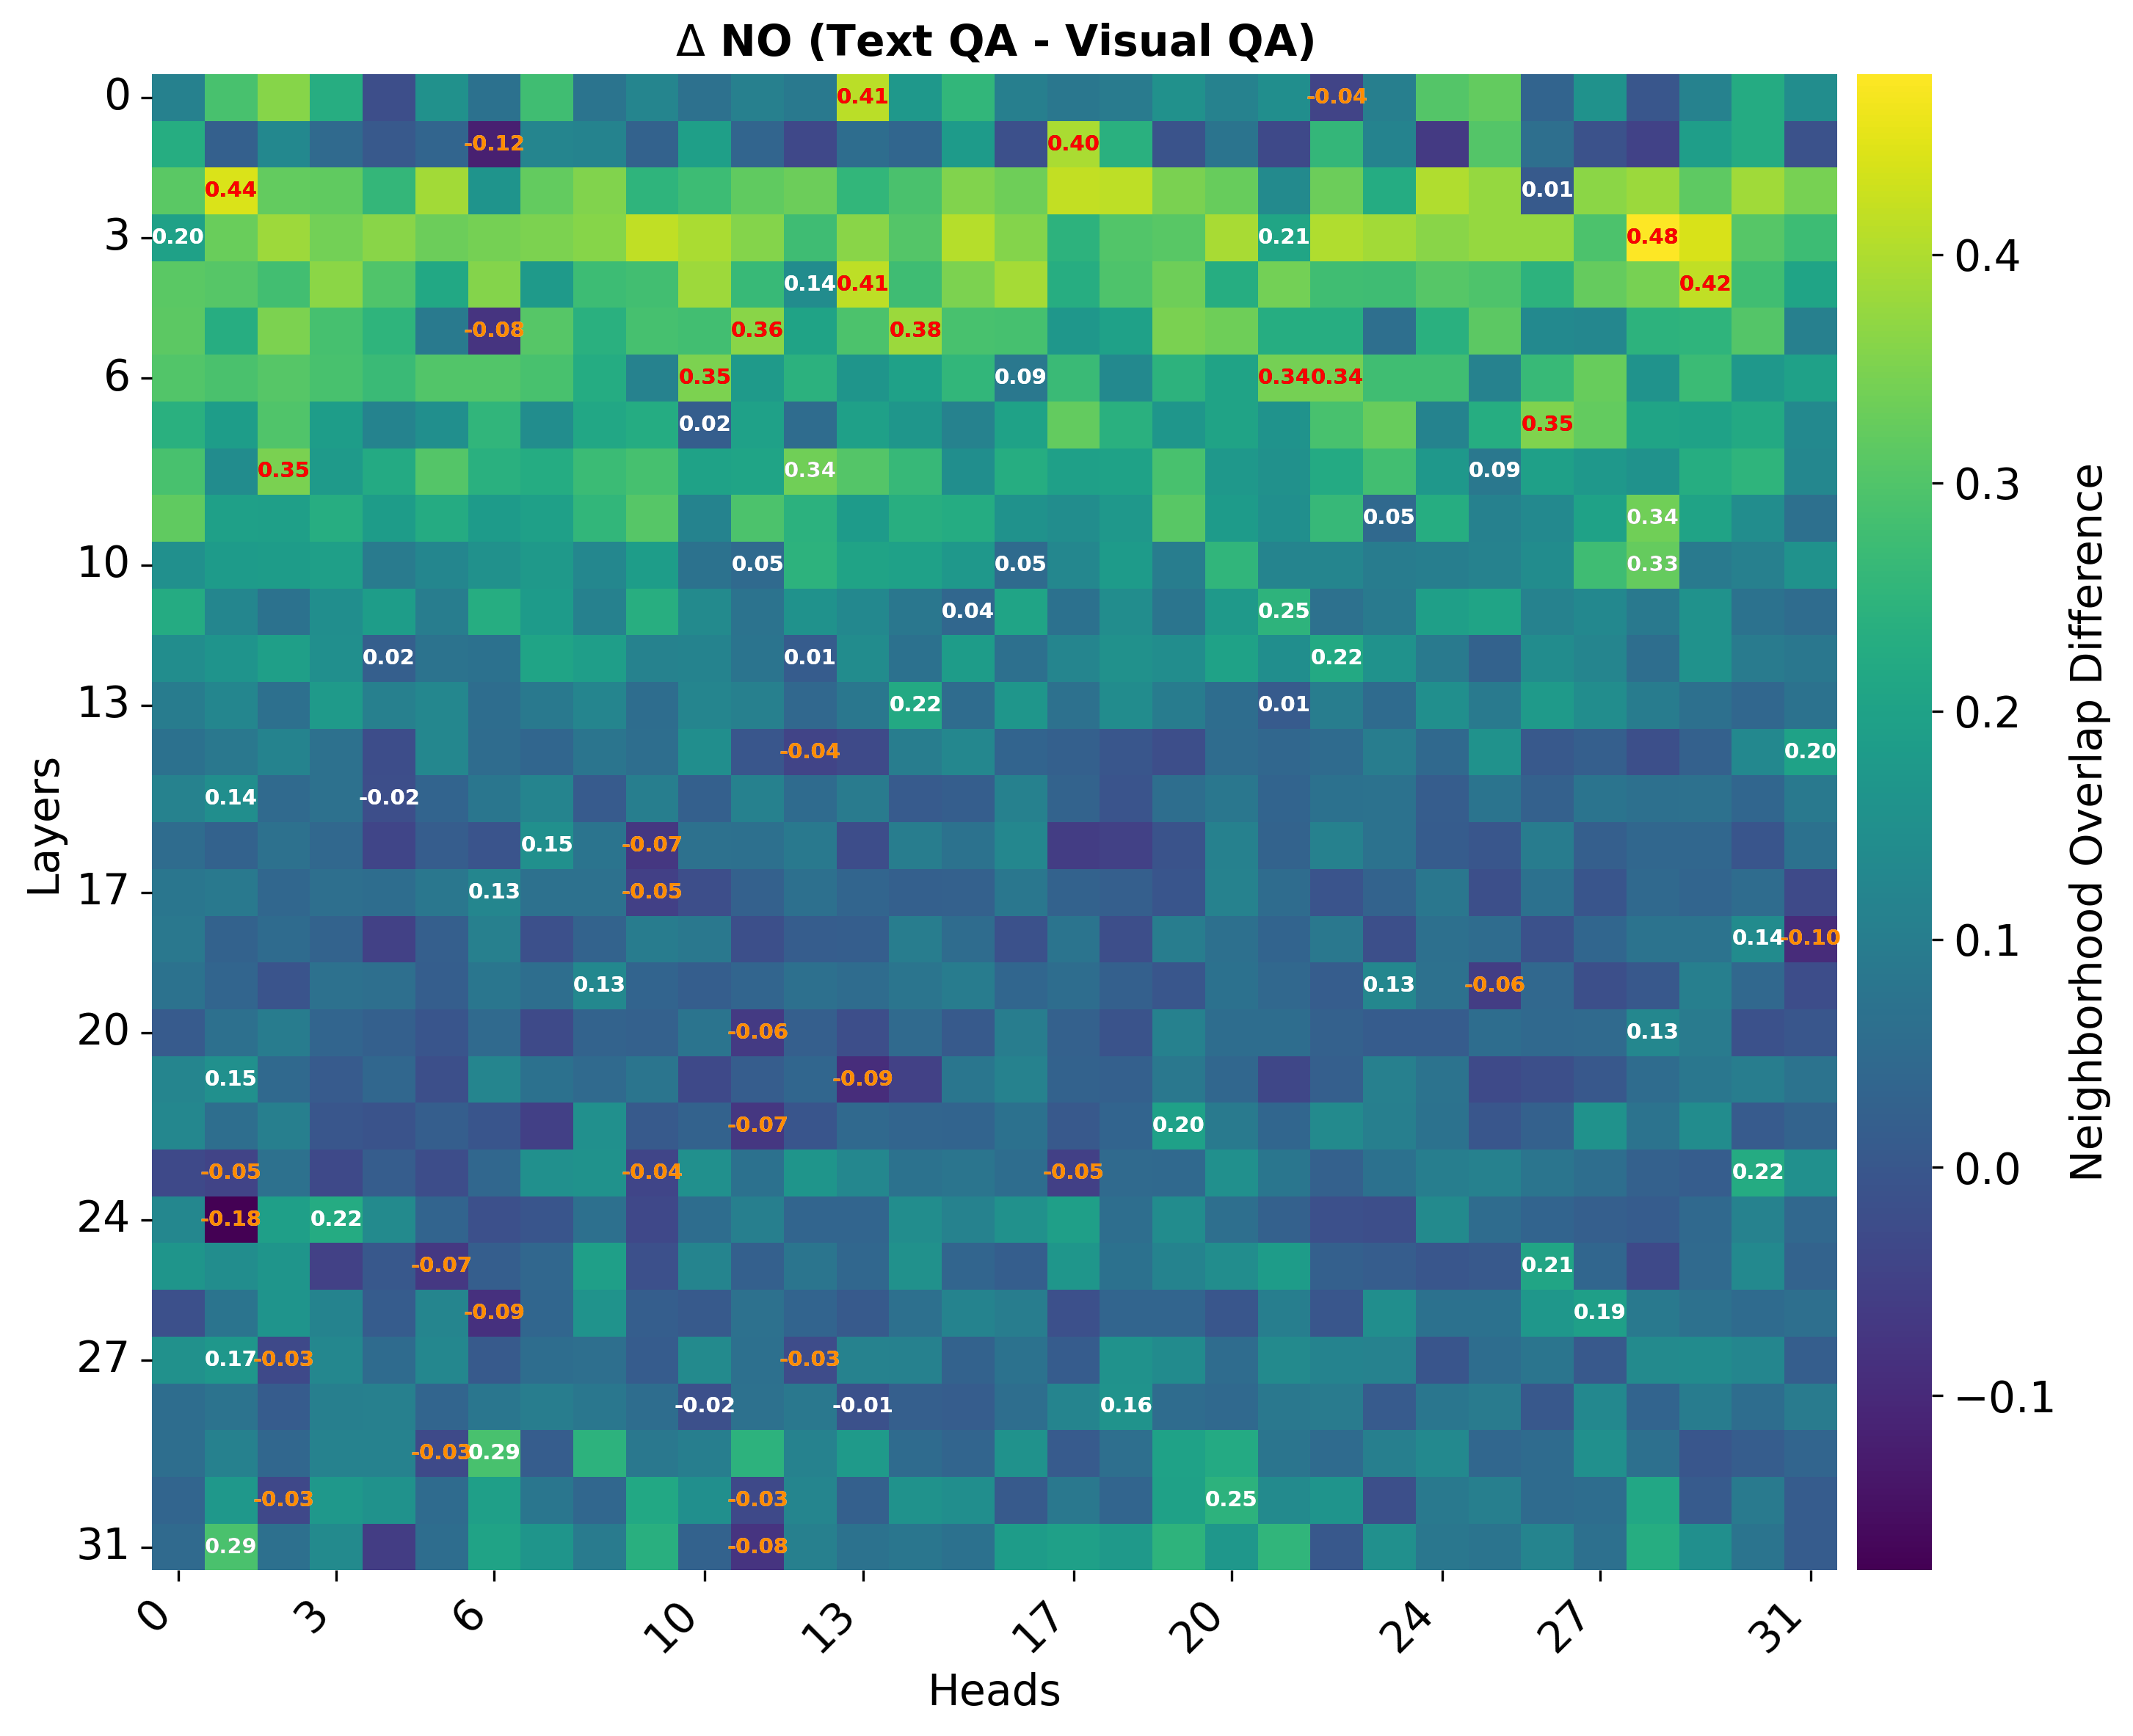
\includegraphics[width=\textwidth]{../images/chapter3/similarity_matrix_cocoqa_txt_minus_cocoqa_img_heads_projection_last_neighborhood_overlap.png}
    \end{subfigure}
    \vspace{-0.25cm}
    \caption{
        Head-wise NO between fine-tuned and pretrained LLaVA. 
        Annotations mark extreme values (white: top/bottom 5\% within layer; red: global top 5\%; orange: global bottom 5\%). 
        (a) Text (left) and visual (right) QA on COCOVQA. 
        (b) Text-multimodal difference (negative: higher multimodal similarity; positive: higher text similarity).
    }
    \label{fig:heads_wise_similarity_cocovqa}
\end{figure}

\paragraph{Impact of visual instruction tuning on representation similarity.}
Figures~\ref{fig:layer_wise_similarity_cocovqa}, \ref{fig:heads_wise_similarity_cocovqa} and \ref{fig:layer_wise_similarity_cocovqa_mean_heads} jointly indicate that visual instruction tuning alters the backbone primarily in the early-mid layers. The sharper similarity drop for multimodal inputs in this region suggests that the effect of visual instruction tuning on the LLM-backbone of LLaVA is localized in the first half of the network. By contrast, the small text-multimodal differences in deep layers (Figures~\ref{fig:layer_wise_similarity_cocovqa_difference} and \ref{fig:layer_wise_similarity_cocovqa_mean_heads_difference}) indicate that late layers mainly coordinate information for next-token prediction, especially on QA. Because the analyzed representations are last-token embeddings and the datasets contain equivalent content in different modalities, these results hint that the initial layers are responsible for multimodal integration. The modest differences in the first two layers may reflect a shared role (e.g., question parsing) prior to strong modality-specific processing. These results contrast with prior work on LLMs \cite{doimoRepresentationLandscapeFewShot} where the representations in the late layers changed the most due to fine-tuning.

Fine-tuning updates the model's weights and thus its internal representations. The reduction in similarity on text is consistent with the fine-tuned model's stronger instruction-following (Table~\ref{tab:benchmark_comparison}). The lower similarity on multimodal data is expected since visual instruction tuning enables the model to understand images.

The rise in the text-multimodal difference (Figures~\ref{fig:layer_wise_similarity_cocovqa_difference} and \ref{fig:layer_wise_similarity_cocovqa_mean_heads_difference}) in the early layers indicates that text retains greater stability than multimodal features (text representations get more and more similar than the multimodal representations). This supports the hypothesis that in the initial layers the model progressively incorporates visual information.

Head-wise results (Figure~\ref{fig:heads_wise_similarity_cocovqa}) suggest the presence of \emph{modality-agnostic} heads, where similarity values are comparable across modalities. These may correspond to heads that serve similar functions regardless of modality, such as interpreting the question or generating the answer. In contrast, heads with the largest positive differences may indicate strong specialization in multimodal understanding, whereas those with the largest negative differences may reflect enhanced text-specific processing. The head-wise modality differences (Figure~\ref{fig:heads_wise_similarity_cocovqa_difference}) show that visual instruction tuning affects all heads, with its strongest concentration in the early layers---though not in tightly clustered groups---consistent with the layer-wise analysis.

\section{Geometry After Fine-Tuning: Intrinsic Dimension}\label{sec:geometric_reorganization}

Having localized where representations change via similarity, this section investigates whether fine-tuning also alters the data manifold geometry of those representations. We estimate the intrinsic dimension for embeddings extracted from COCOVQA under text and visual QA (setup as in Section~\ref{sec:question_answering}) and image captioning (prompt as in Section~\ref{sec:modality_gap_experiment_setup}). This tests whether the early-mid layer differences seen in similarity correspond to a systematic geometric reorganization, directly addressing the thesis goal of identifying \emph{where and how} visual instruction tuning modifies the LLM backbone.

Figure~\ref{fig:intrinsic_dimension_combined} shows that, for the pretrained and fine-tuned models, ID starts at about 13-17 in shallow layers and then decreases with depth. In the fine-tuned model, text QA maintains consistently higher IDs than multimodal tasks. With the exception of small fluctuations in text-only representations, all tasks peak early (layer$\sim$4; $\sim$16-18), dip near layer 10, rise again mid-network, and then decline steadily after layer$\sim$20, stabilizing around 9-10 in the deepest layers, where curves for all tasks converge. 

\begin{figure}
    \centering
    \begin{subfigure}[t]{0.65\textwidth}
        \centering
        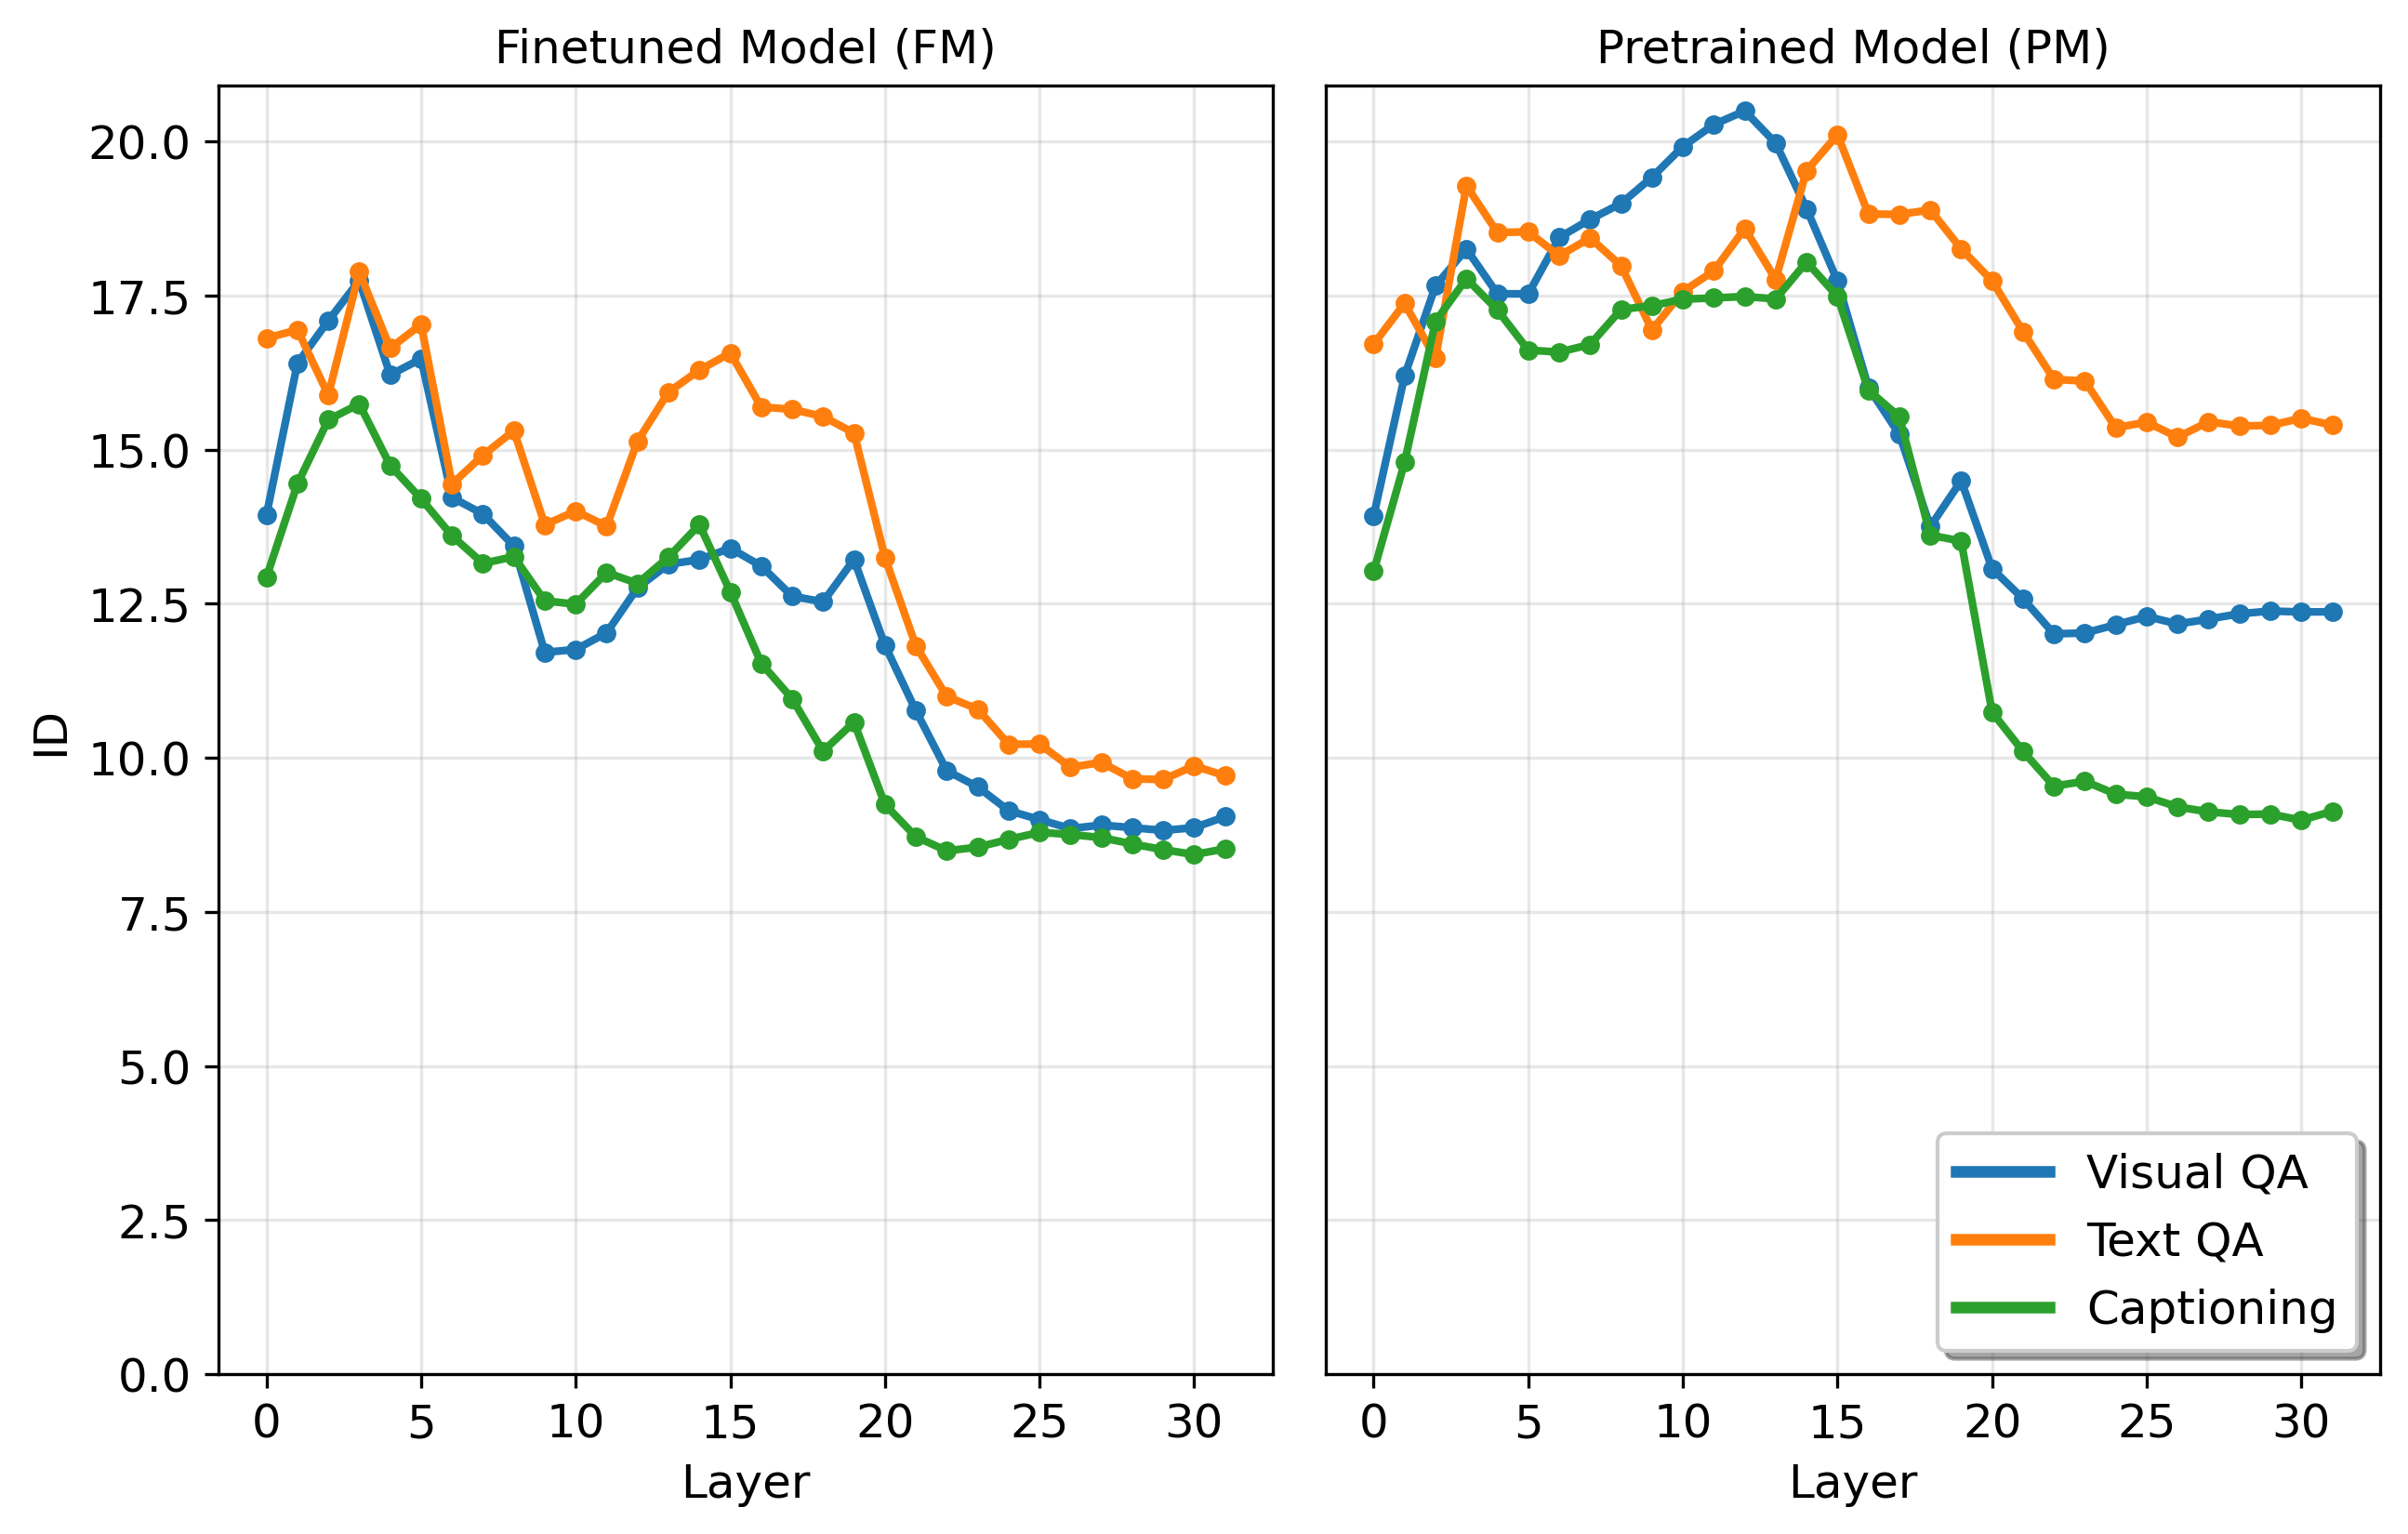
\includegraphics[width=\textwidth]{../images/chapter3/model_data_measures_intrinsic_dimension_output_layer_last.png}
        \vspace{-0.65cm}
        \caption{
            % leave caption blank
        }
        \label{fig:intrinsic_dimension_combined}
    \end{subfigure}
    \begin{subfigure}[t]{0.34\textwidth}
        \centering
        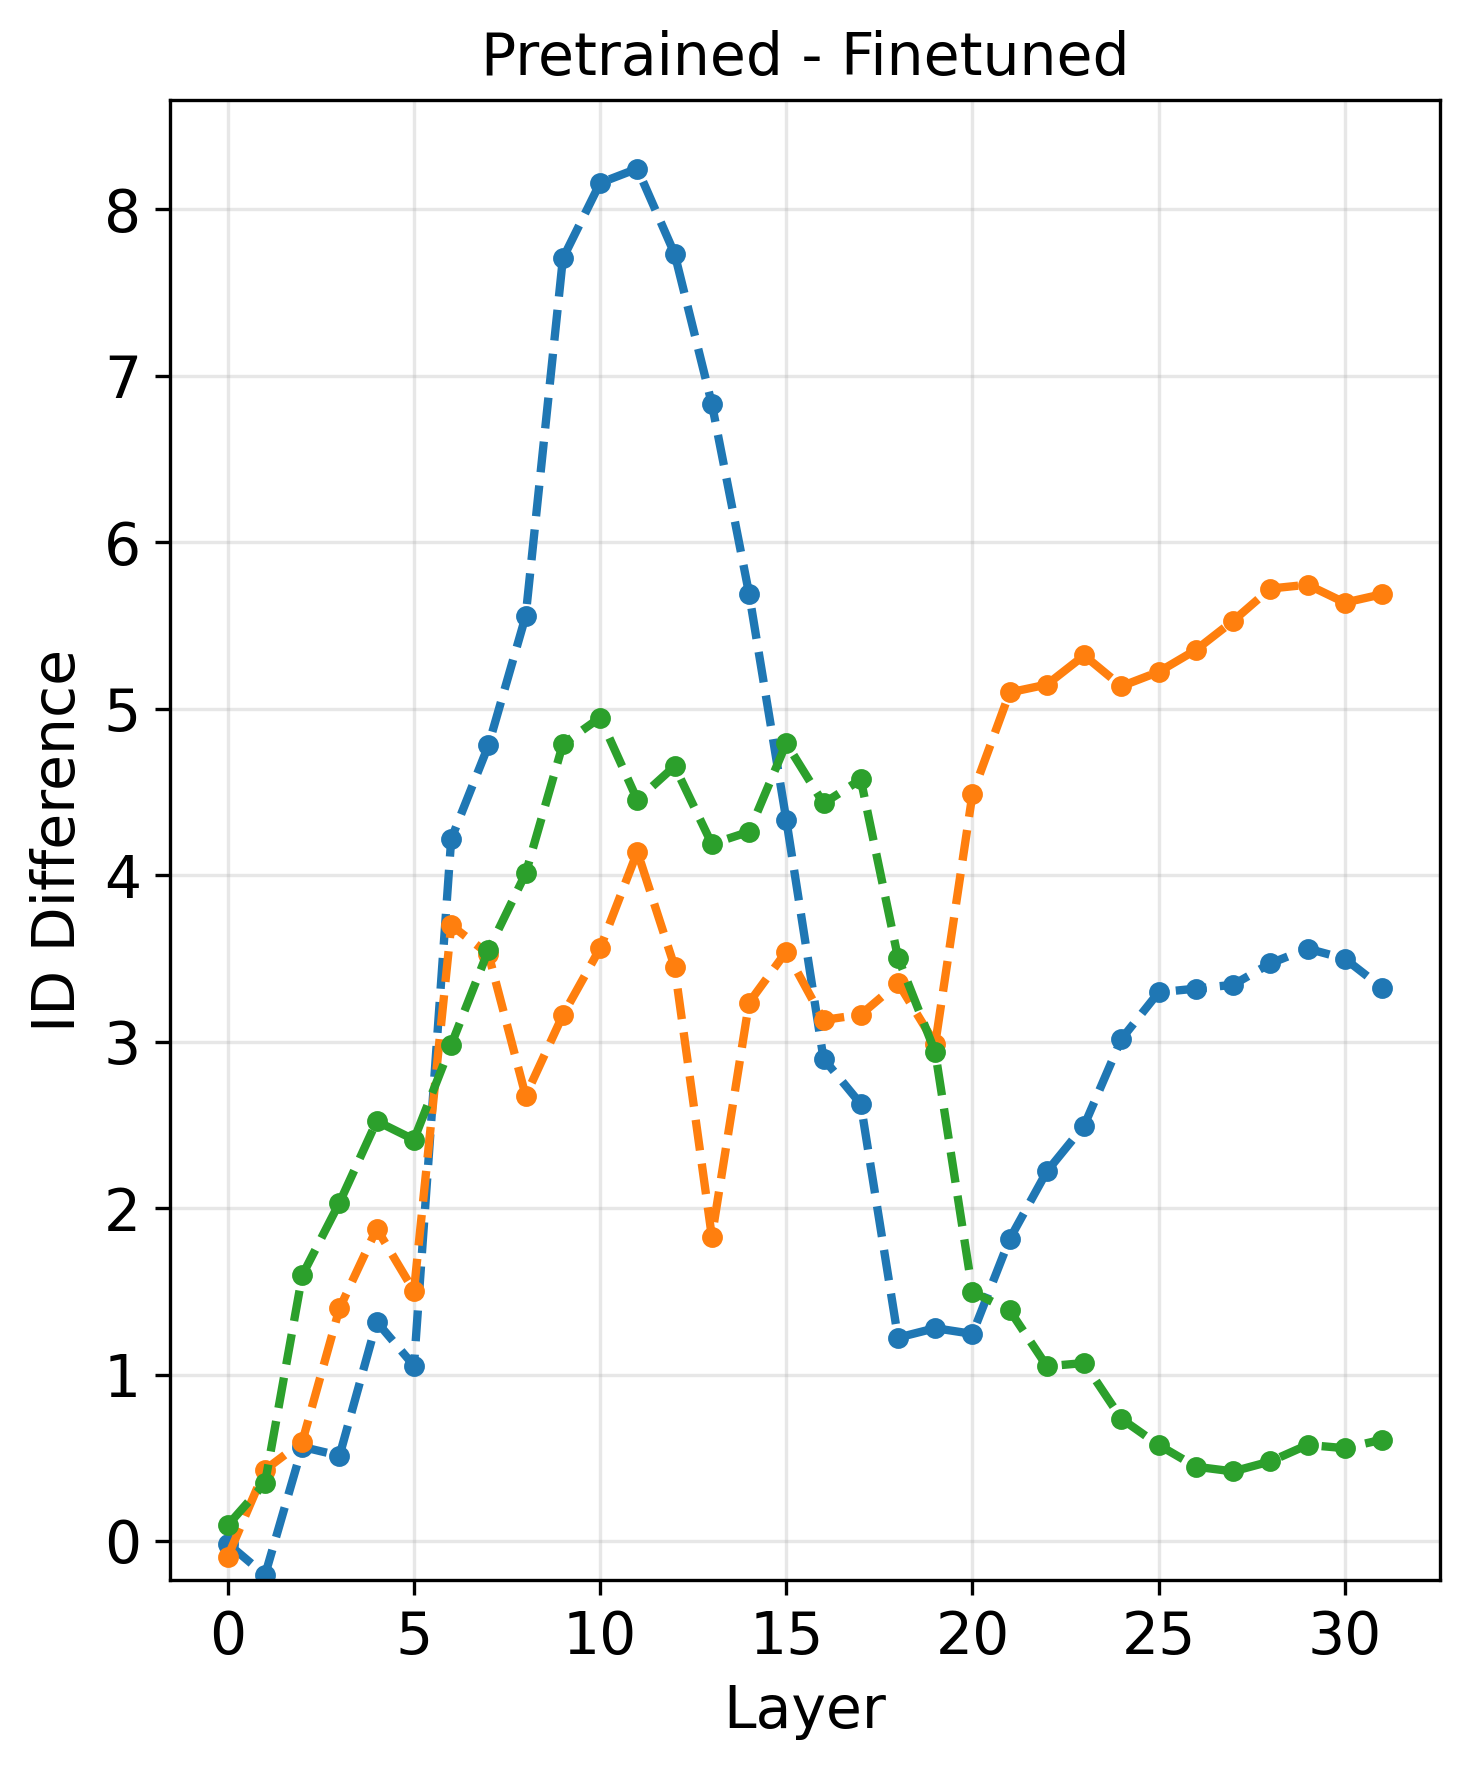
\includegraphics[width=\textwidth]{../images/chapter3/model_data_measures_differences_intrinsic_dimension.png}
        \vspace{-0.65cm}
        \caption{
            % leave caption blank
        }
        \label{fig:intrinsic_dimension_difference}
    \end{subfigure}
    \vspace{-0.3cm}
    \caption{
        Intrinsic dimension analysis for text QA (orange), visual QA (blue), and image captioning (green) on COCOVQA. 
        (a) Finetuned model (left) and pretrained model (right). Higher values indicate higher-dimensional (less compact) representations.
        (b) ID difference (pretrained $-$ fine-tuned). Positive values mean the pretrained model has higher ID.
    }
    \label{fig:intrinsic_dimension}
\end{figure}

In the pretrained model, the second half of the network follows a similar downward trend, but early layers differ: multimodal IDs increase steadily while IDs for text QA and image captioning either fluctuate or grow more slowly. Peaks occur later (layers$\sim$13-16), in contrast to the early peak in the fine-tuned model, with visual QA reaching $\sim$21 above the maxima of the other tasks. By the final layers, IDs remain larger overall than in the fine-tuned model, and the three tasks are still separated by $\sim$3 units.

The difference panel in Figure~\ref{fig:intrinsic_dimension_difference} makes the effect of fine-tuning explicit: IDs are generally \emph{lower} after fine-tuning, especially in mid layers for multimodal inputs. For visual QA, the gap peaks near layer$\sim$12 where the ID difference is $\sim$8, then decreases and rises at a slower rate before stabilizing. Beyond layer$\sim$20, differences settle around 5-6 for text QA, 3-4 for visual QA, and near zero for captioning. Notably, for purely textual inputs, IDs in the pretrained model remain higher than in the fine-tuned model throughout depth, with the largest compression appearing toward the end.

A complementary analysis in Figure~\ref{fig:dataset_entropy} of the appendix uses \emph{dataset entropy}~\cite{skeanLayerLayerUncovering2025}, an information-theoretic analogue of ID. It is defined as the Shannon entropy of the normalized eigenvalue spectrum of the Gram matrix built from centered and normalized dataset representations. Higher entropy indicates a more diffuse spread of variance across eigen-directions, corresponding to less compact representations and more diverse features. Its layer-wise pattern broadly mirrors (though not identical) the ID curves: entropy differences (pretrained $>$ fine-tuned) peak around layers 10-12 for multimodal data, then converge in deep layers (text $\approx 0.08$, multimodal $\approx 0.05$, and captioning $\approx 0$, with a residual $\approx 0.04$ in the final layer).

\paragraph{What ID reveals about fine-tuning.}
The change in ID and dataset entropy in Figures \ref{fig:intrinsic_dimension} and \ref{fig:dataset_entropy} support the hypothesis that the early-mid layers are the ones changing the most in the LLaVA LLM-backbone due to visual instruction tuning, and is consistent with the NO and linear CKA similarity analysis shown in Section~\ref{sec:representational_similarity}. The compression observed in these layers aligns with prior work on autoregressive transformers using entropy-based measures~\cite{skeanLayerLayerUncovering2025}, and the hump-shaped ID profile of the pretrained model matches reports for LLaMA models~\cite{doimoRepresentationLandscapeFewShot}. Fine-tuning \emph{compresses} the representation manifolds (lower ID/entropy), most strongly for multimodal inputs in mid layers, and with smaller but persistent reductions in late layers (particularly for text). In the deepest layers, IDs across tasks converge toward a common, compact regime, consistent with these layers chiefly coordinating information for next-token prediction. This supports the hypothesis that visual instruction tuning primarily injects and integrates visual grounding in the first half of the backbone, while later layers act as shared decoders across modalities.

\section{Modality Gap After Fine-Tuning: Alignment vs.\ Separation}

Having established \emph{where} the backbone changes (via similarity) and \emph{how} geometry is reorganized (via ID) \emph{between the model's checkpoints}, we now analyze the \emph{relationship between data modalities within models' checkpoints}. Using the setup in Section~\ref{sec:modality_gap_experiment_setup}, we quantify the text-image \emph{modality gap} with two complementary views: (i) we examine the directional alignment between the most contextualized text and image embeddings by computing the cosine similarity between them, and (ii) analyze the cluster separation and homogeneity with advanced density peak clustering.

\paragraph{Directional alignment.}

Figure~\ref{fig:cosine_similarity_text_image} shows that, for both captioning (left) and visual QA (right), cosine similarity is initially low in shallow layers, increases from about layer 10, and peaks in the deepest layers. Across most deeper layers, the pretrained model exhibits higher alignment than the fine-tuned model; the fine-tuned model briefly exceeds it in the earliest layers and again at the final layer for captioning.

\begin{figure}
    \centering
    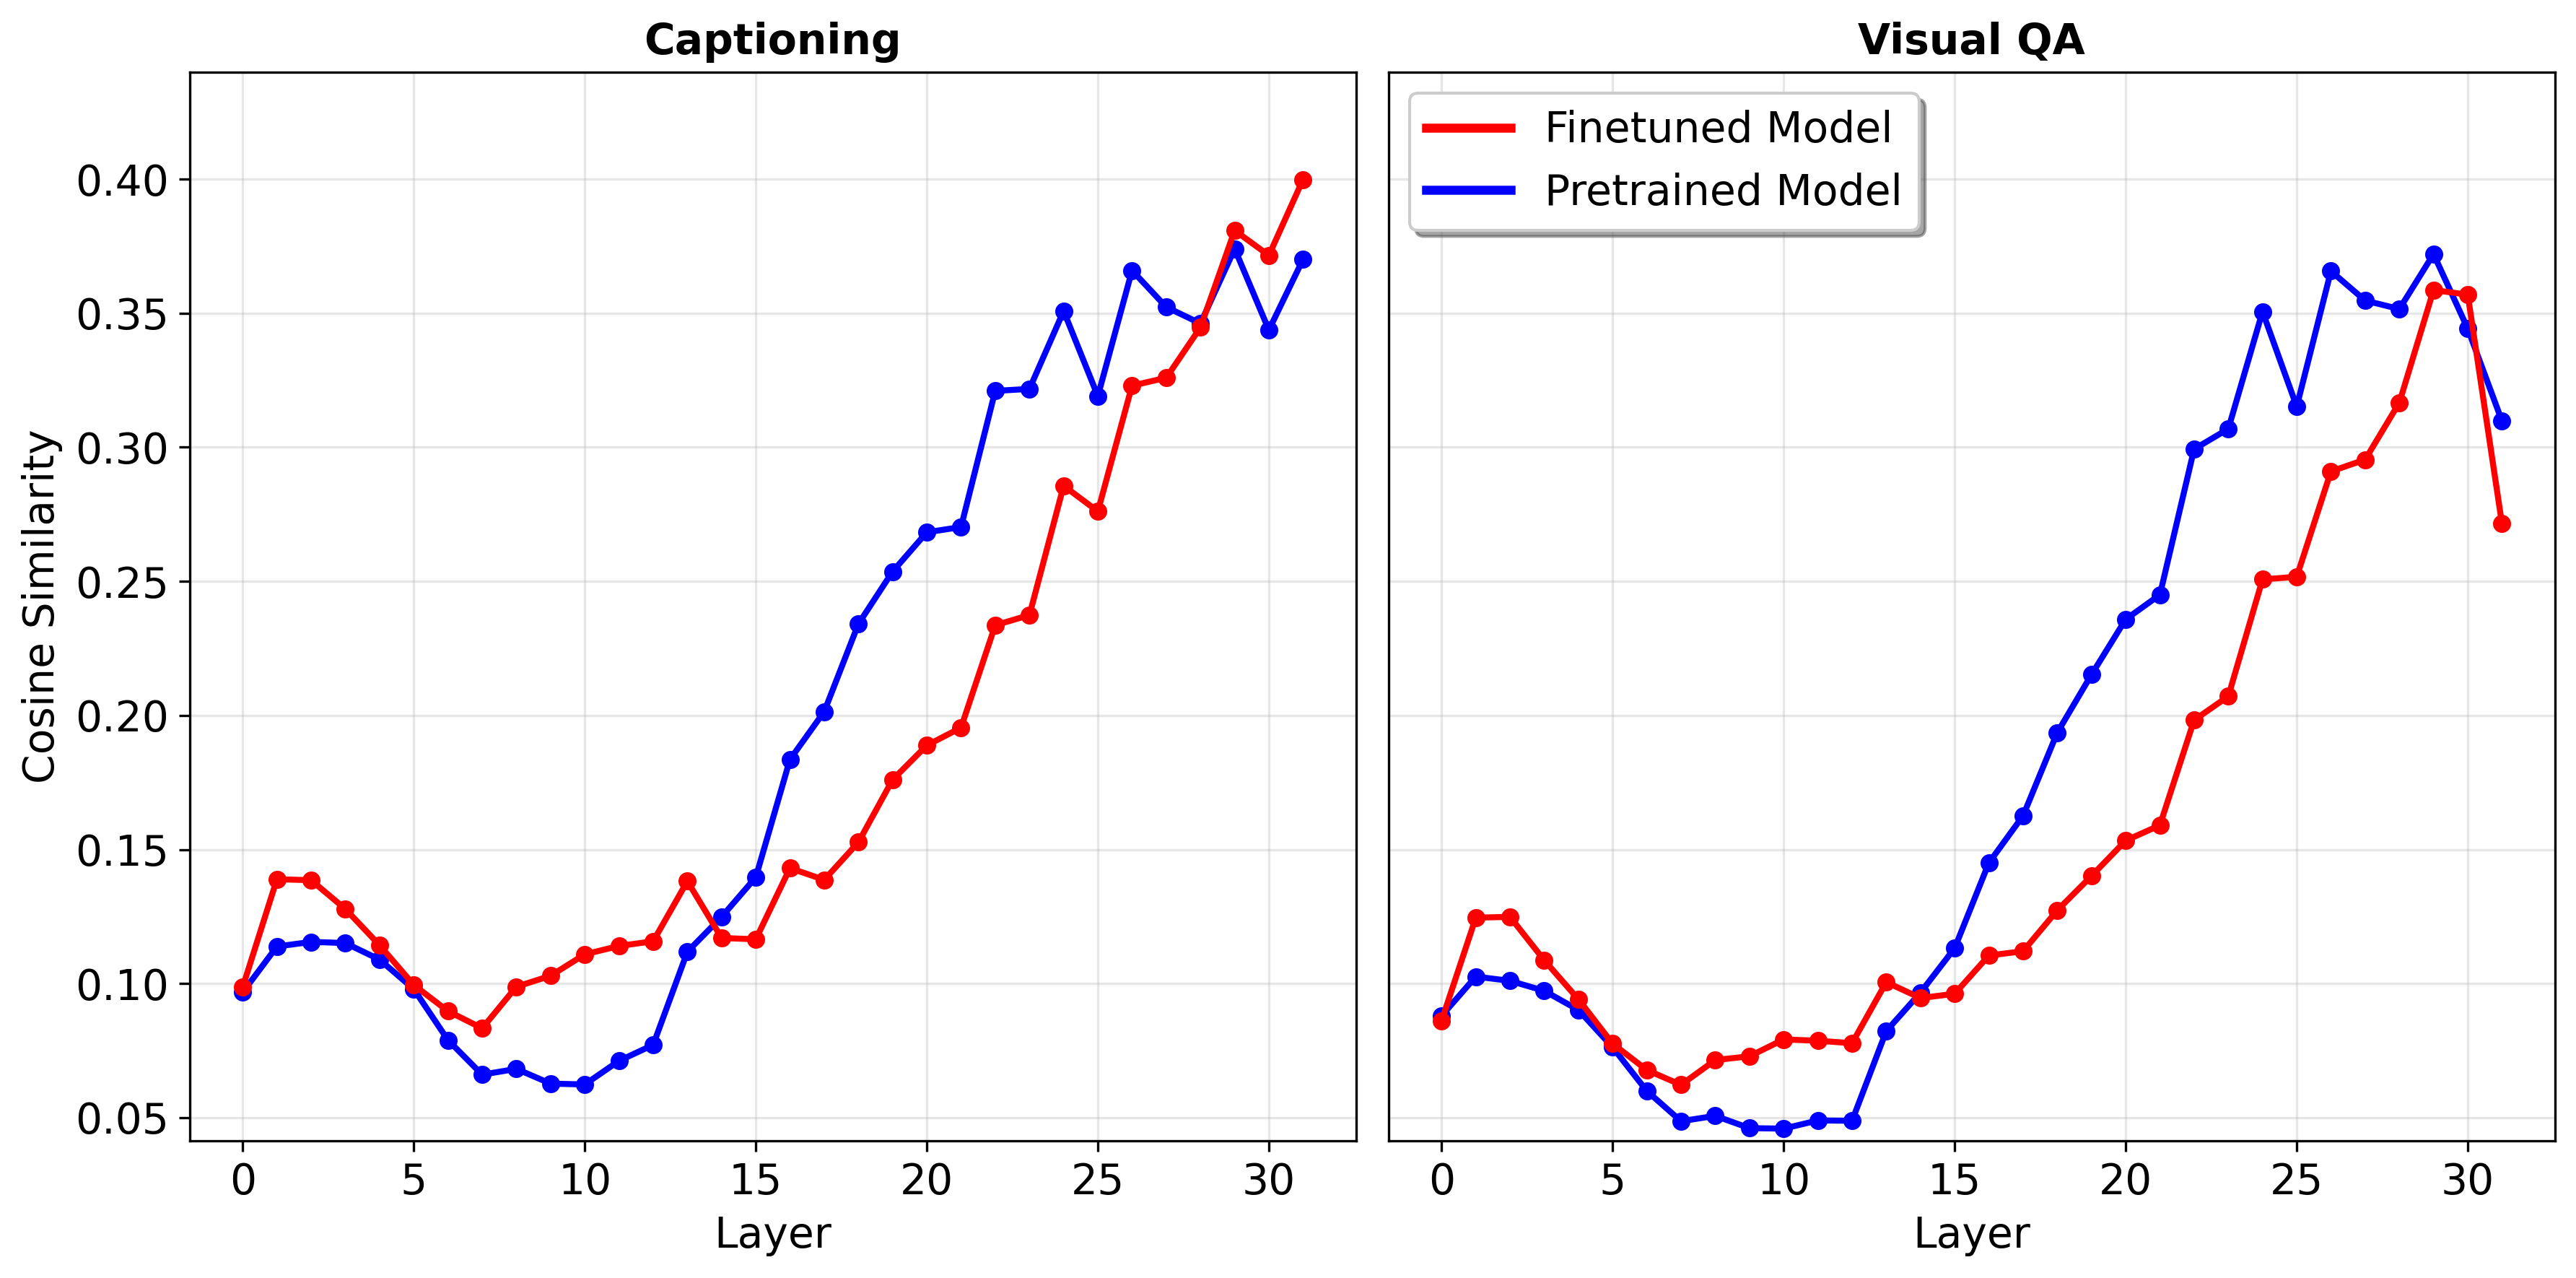
\includegraphics[width=\textwidth]{../images/chapter3/modalities_similarities_cosine_similarity_output_layer.png}
    \caption{
        Cosine similarity between the most contextualized text and image representations of the fine-tuned (red) and pretrained (blue) LLaVA, for image captioning (left) and visual QA (right) on the multimodal subset of COCOVQA. Higher values indicate stronger directional alignment.
    }
    \label{fig:cosine_similarity_text_image}
\end{figure}

\begin{figure}
    \centering
    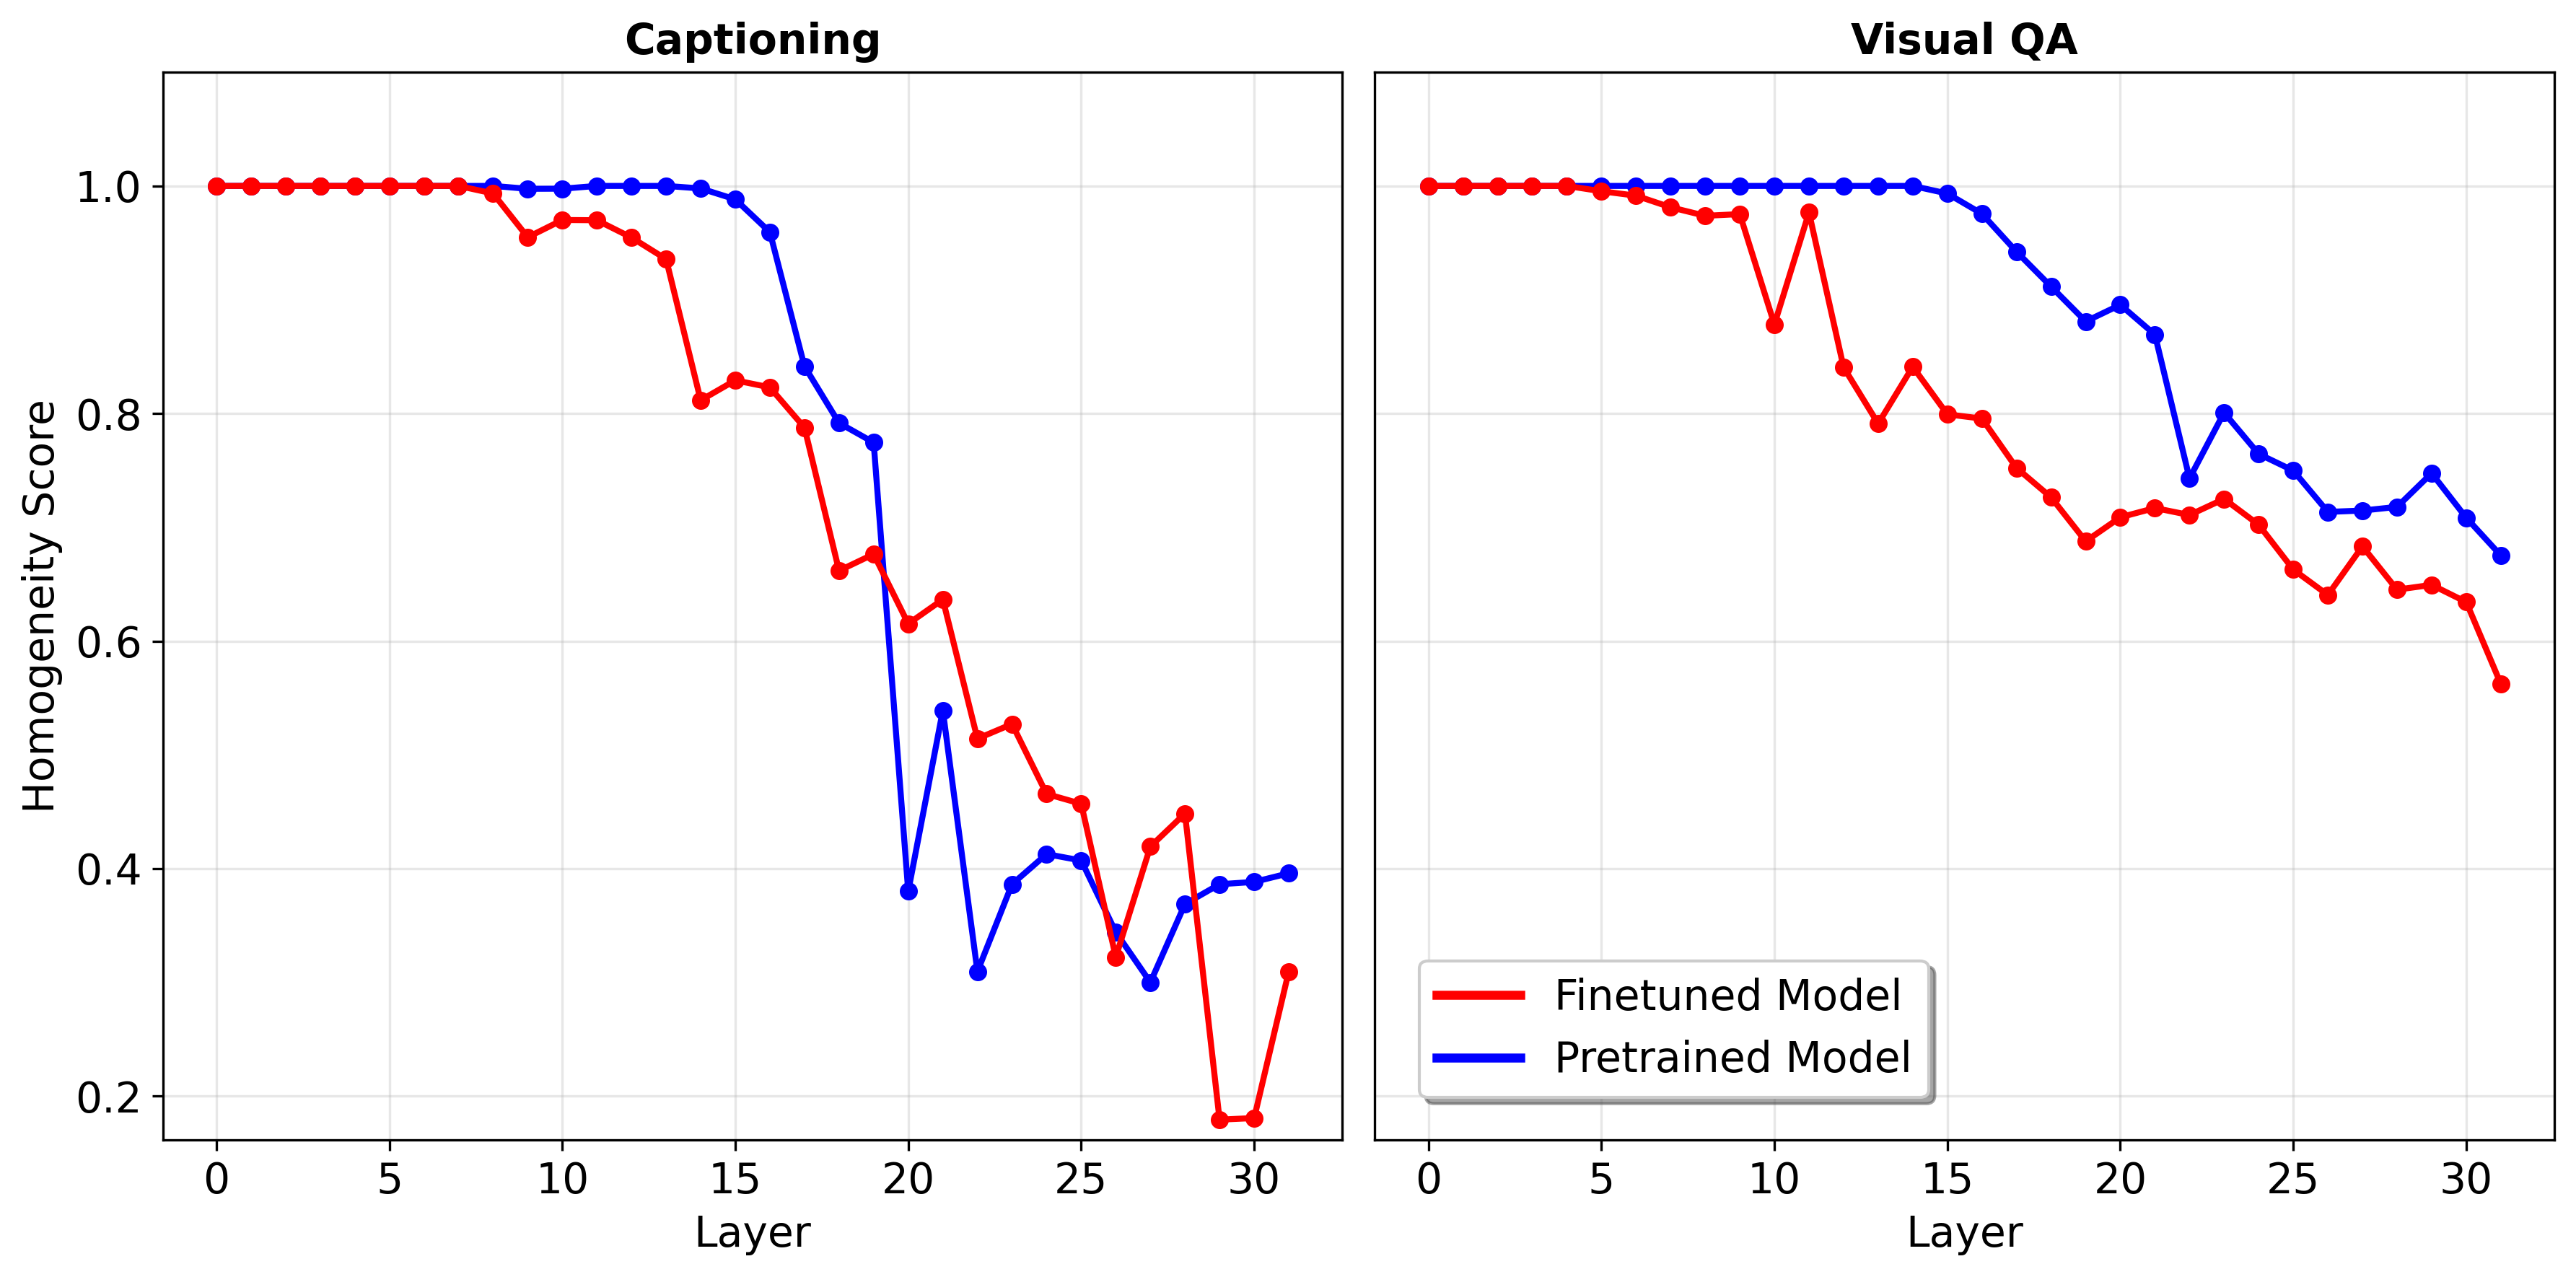
\includegraphics[width=\textwidth]{../images/chapter3/modalities_similarities_homogeneity_score_cosine_output_layer.png}
    \caption{
        Homogeneity after clustering text and image embeddings together (same tasks as in Figure~\ref{fig:cosine_similarity_text_image}). A value of~1 indicates perfectly separated modality clusters; lower values indicate stronger mixing.
    }
    \label{fig:homogeneity_score_text_image}
\end{figure}


\paragraph{Cluster homogeneity.}
Figure~\ref{fig:homogeneity_score_text_image} reports homogeneity after clustering text and image embeddings together with ADP. Scores start near 1.0 (well-separated modality clusters) and then decline with depth, with a sharper drop beginning around layers 10-12, mirroring the rise in cosine similarity. For visual QA (right), the pretrained model maintains higher homogeneity than the fine-tuned model across the network, with the largest gap roughly in layers 12-23. For captioning (left), the pretrained curve remains near 1.0 until about layer 15 and then falls more rapidly than the fine-tuned curve; final values are $\sim$0.40 (pretrained) vs.\ $\sim$0.30 (fine-tuned), both lower than in QA.

\paragraph{Effect of fine-tuning on the modality gap.}
The directional alignment (cosine similarity; Figure \ref{fig:cosine_similarity_text_image}) and the clustering structure (homogeneity score; Figure \ref{fig:homogeneity_score_text_image}) follow prior observations for LLaVA's modality gap \cite{serraNarrowGateLocalizeda}. Cosine similarity increases with depth in both pretrained and fine-tuned models, indicating that text and image representations are nearly orthogonal in early layers and become progressively more aligned in mid-to-late layers. Relative to the pretrained model, fine-tuning slightly increases alignment in early layers, whereas in late layers the gap is slightly larger (the pretrained model tends to show higher similarity), consistent with reports that a larger gap can correlate with better downstream performance \cite{liangMindGapUnderstanding2022} (see Table \ref{tab:benchmark_comparison}).

The homogeneity score declines with depth (Figure \ref{fig:homogeneity_score_text_image}), meaning that modality-pure clusters (score $\approx$ 1) in shallow layers become increasingly mixed in deeper layers. On the question-answering task, mid-layer homogeneity is lower for the fine-tuned model than for the pretrained model, suggesting stronger mixing, and thus a smaller gap, in that region. In the final layers, the two tasks diverge and do not yield a single, task-independent conclusion.

\paragraph{Summary and scope.}
Directional alignment (cosine similarity) and cluster homogeneity do not exhibit a single, consistent pattern across tasks. In early layers, fine-tuning slightly increases text-image alignment while modality clusters remain well separated. Deeper in the network, alignment is generally lower for the fine-tuned model; however, cluster separability diverges by task-embeddings mix more for QA and slightly less for captioning. These findings are specific to the tasks evaluated, our setting and to the specific fine-tuning setup of LLaVA (one-epoch update of the LLM backbone).

\section{Task-Level Validation via Layer Patching}

This section applies the patching protocol from Section~\ref{sec:functional_localization_via_layer_patching} to \emph{text VQA}, \emph{visual VQA}, and \emph{image captioning} (all built from COCOVQA). We form \emph{hybrid} models by replacing subsets of the pretrained backbone with the corresponding fine-tuned layers using two schemes: (i) \emph{cumulative} patching and (ii) \emph{sliding-window} patching. In the cumulative scheme, we patch from the start to the end of the network and denote by $\ell$ the \emph{last} included layer index (0-indexed), i.e., layers $[0{:}\ell]$ are taken from the fine-tuned model. In the sliding-window scheme, we patch a contiguous window of size $w$ starting at index $\ell$, i.e., layers $[\ell{:}\ell{+}w]$ are patched.

\subsection{Question Answering}

Accuracy increases as more fine-tuned layers are \emph{cumulatively} patched (Figure~\ref{fig:accuracy_question_answering_cumulative}). On \emph{visual} QA, performance rises with $\ell$: 19\% above the pretrained reference (0.42) at $\ell=2$; $85-98$\% of the fine-tuned reference (0.66) for $\ell=4-12$; and from about 12 layers onward, the hybrid matches or exceeds the fine-tuned model. When all backbone layers are patched \emph{except} the final LM head (output layer), accuracy reaches 103\% of the fine-tuned model. On \emph{text} QA, accuracy stays at or slightly below the pretrained reference for shallow patches, then increases after 14 layers and eventually matches the fine-tuned model.

\begin{figure}
    \centering
    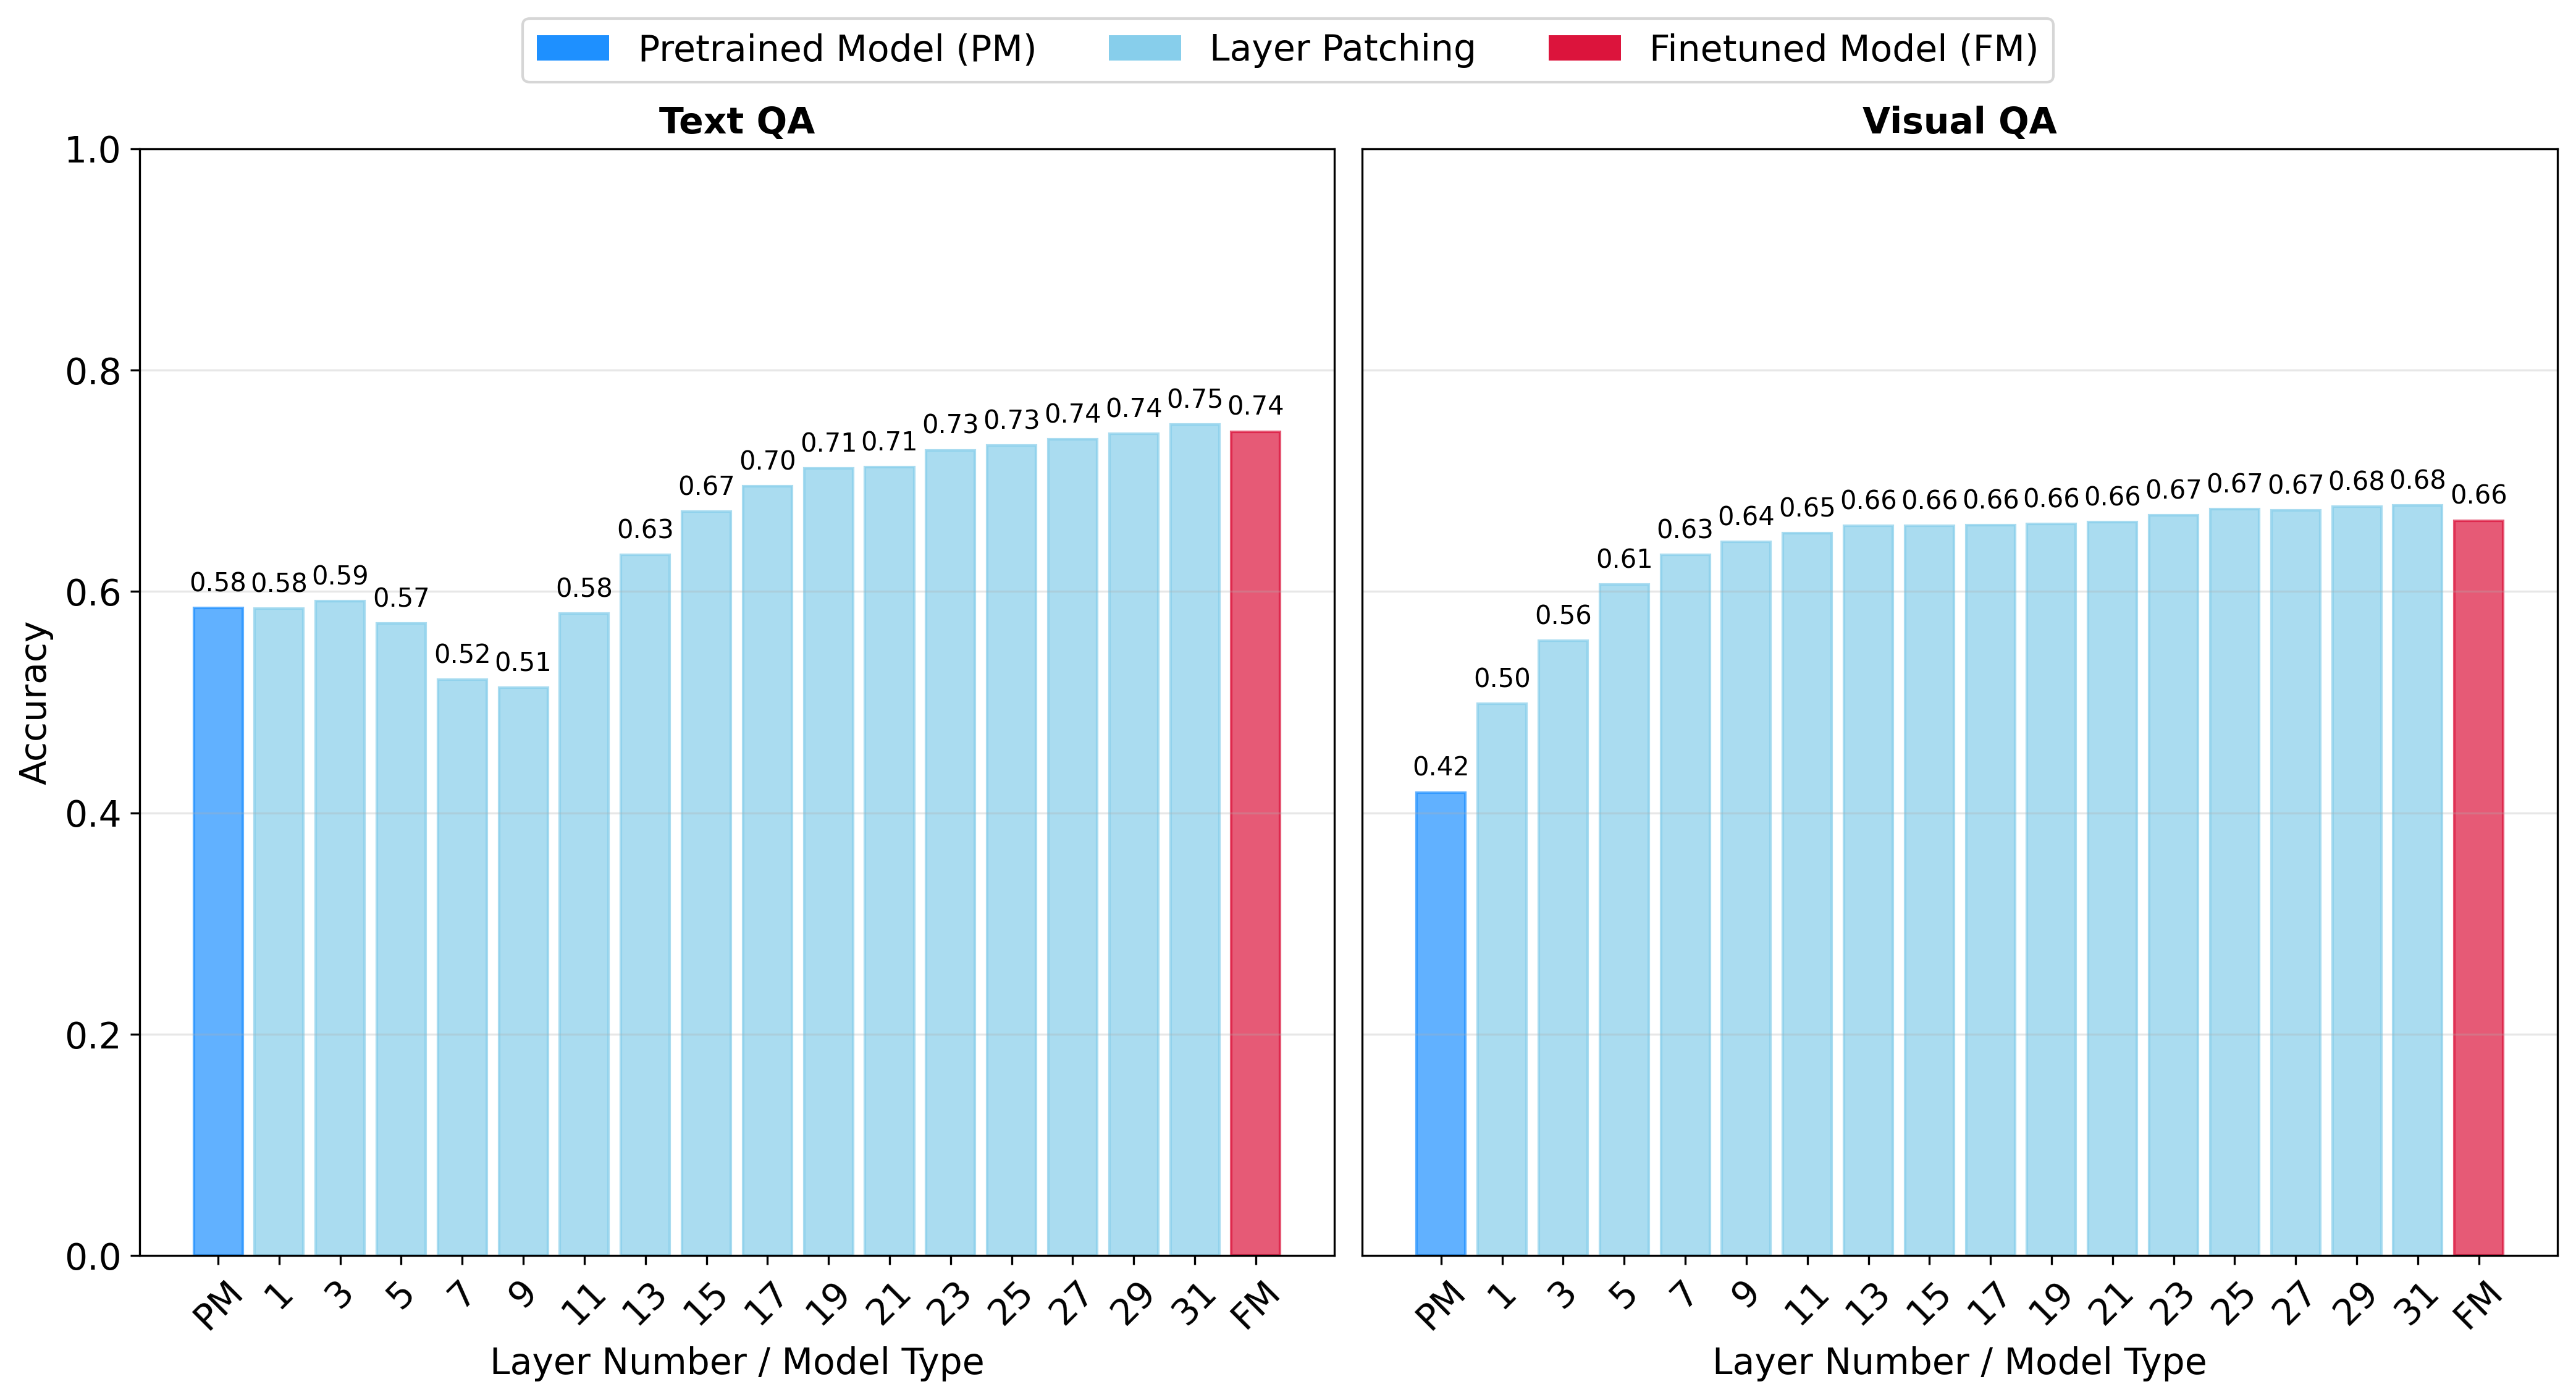
\includegraphics[width=\textwidth]{../images/chapter3/transplanting_layers_qa_benchmarking_two_parts_s2.png}
    \caption{
        COCOVQA question-answering accuracy for hybrids formed by \emph{cumulatively patching} layers $[0{:}\ell]$ from the fine-tuned backbone into the pretrained backbone (light-blue bars). The x-axis is $\ell$. Left: text-only QA. Right: visual QA. Blue and red bars denote the pretrained (PM) and fine-tuned (FM) references, respectively.
    }
    \label{fig:accuracy_question_answering_cumulative}
\end{figure}

For a complementary view, the \emph{sliding-window} results (Appendix; Figure~\ref{fig:accuracy_question_answering_sliding_window}) patch a single layer at a time ($w=1$) starting at index $\ell$. Effects are small and localized: on text QA, accuracies hover near the pretrained reference; on visual QA, early-layer patches yield a modest bump that fades in mid-to-deep layers. No single-layer patching approaches the fine-tuned reference.

\subsection{Image Captioning}

Image captioning shows the same monotonic trend under \emph{cumulative} patching. CIDEr is near zero for the pretrained model and remains small for shallow patches ($\ell=1-7$); it rises sharply for $\ell \approx 9-15$ and then climbs more gradually, peaking at $0.81$ for $\ell=31$ (all backbone layers are patched except the LM head), close to the fine-tuned reference ($0.82$). CLIP-Score follows the same pattern, moving from $0.14-0.16$ for shallow patches to $0.23$ for deep patches, slightly above the fine-tuned reference ($0.22$) and well above the pretrained reference ($0.15$).

\begin{figure}
    \centering
    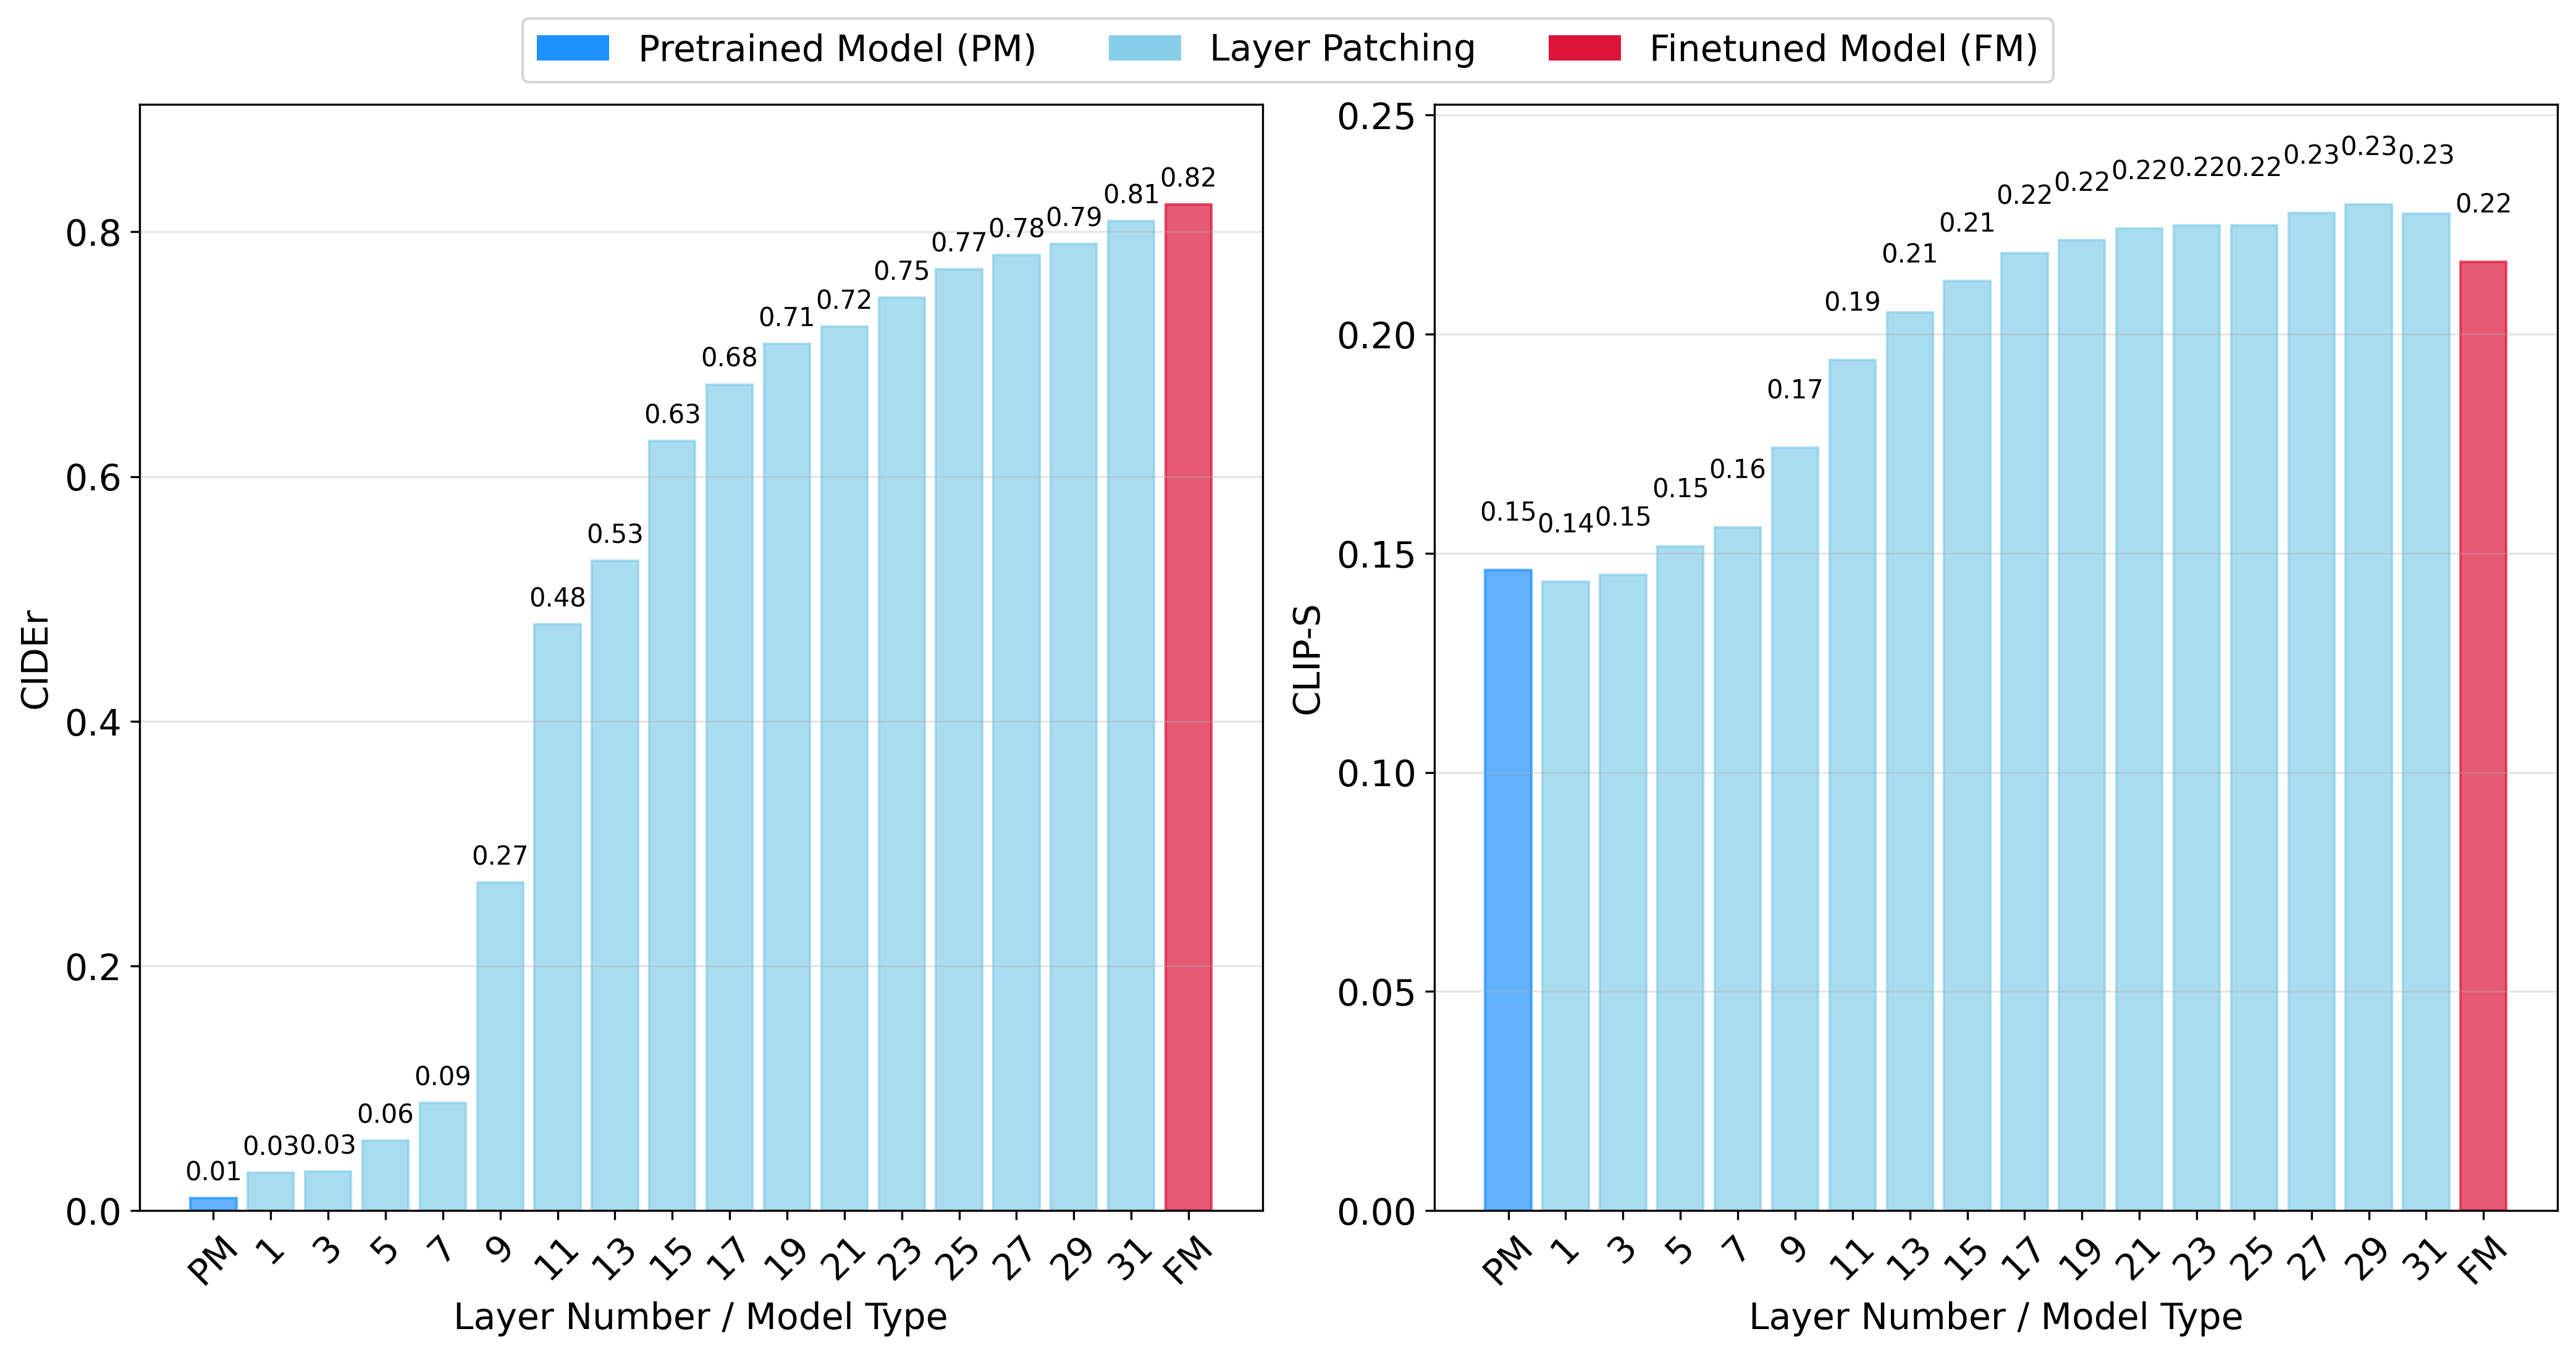
\includegraphics[width=\textwidth]{../images/chapter3/transplanting_layers_caption_benchmarking_combined_incremental_tokens100.png}
    \caption{
        Image captioning performance under \emph{cumulative} patching of layers. Similar to Figure~\ref{fig:accuracy_question_answering_cumulative}. Left: CIDEr. Right: CLIP-Score.
    }
    \label{fig:cider_clip_score_image_captioning_cumulative}
\end{figure}

The complementary \emph{sliding-window} analysis (Appendix; Figure~\ref{fig:cider_clip_score_image_captioning_sliding_window}) confirms localization: patching a single layer ($w=1$) yields small, position-specific effects (CIDEr peaks around $\sim$0.10-0.11 in early-mid layers; CLIP-Score remains $\sim$0.15-0.16). No single-layer patch approaches the fine-tuned reference.

\paragraph{What patching reveals.}
Cumulative hybrids models (pretrained layers combined with fine-tuned ones) exhibit a clear performance increase followed by a plateau on both QA and image captioning (Figures~\ref{fig:accuracy_question_answering_cumulative} and \ref{fig:cider_clip_score_image_captioning_cumulative}). The steep gains for early-mid layers indicate that visual instruction tuning primarily edits this region, which carries visual understanding and multimodal integration. Beyond that, returns diminish, suggesting late layers chiefly coordinate/decoding for next-token prediction rather than adding multimodal capability. A modest dip on text QA around $\ell \approx 8-10$ (see Figure~\ref{fig:accuracy_question_answering_cumulative}) may also be a consequence of fine-tuning, though evidence is limited. The slight performance excess of the cumulatively patched model that includes all backbone layers except the LM head, relative to the fine-tuned checkpoint, is likely attributable to LM-head updates during fine-tuning (the gain is small). The sliding-window results (Appendix; Figures~\ref{fig:accuracy_question_answering_sliding_window} and \ref{fig:cider_clip_score_image_captioning_sliding_window}) reinforce this picture: improvements concentrate in early-mid layers and are otherwise small. Overall, these task-level outcomes functionally validate the representational findings: instruction tuning embeds visual knowledge mainly in early-mid LLM-backbone depth, while late layers behave as shared decoders across modalities.